\documentclass[12pt,oneside,a4paper]{report}


\usepackage{graphicx}
\usepackage{algorithmicx} 
\usepackage[whole]{bxcjkjatype}
\usepackage{amsmath}%xrightarrow
\usepackage{amsthm}%proof
\usepackage{enumerate}%item
\usepackage{CJKutf8} 
\usepackage{tikz} 
\usepackage{latexsym}
\usepackage[]{algorithm2e}
\usepackage[final]{pdfpages}
\usepackage[T2A,T1]{fontenc}
\usepackage{CJKutf8}

%\newtheorem{name}[count]{NAME}[section]
\newtheorem{example}{EXAMPLE}[section]
\newtheorem{definition}{Definition}[section]
\newtheorem{fact}{Fact}[section]
\newtheorem{proposition}[definition]{Proposition}
\newtheorem{corollary}[definition]{Corollary}
\newtheorem{lemma}[definition]{Lemma}
\newtheorem{theorem}[definition]{Theorem}


\begin{document}

%\title{A Study on Descriptive Patterns Based on Similarity Classes of Individual Constants\\}
%\titleE{\begin{CJK}{UTF8}{ipxm}\begin{CJK}{UTF8}{ipxm}\end{CJK}}
%\author{Wang Ruipeng}
%\date{\today}
%\maketitle
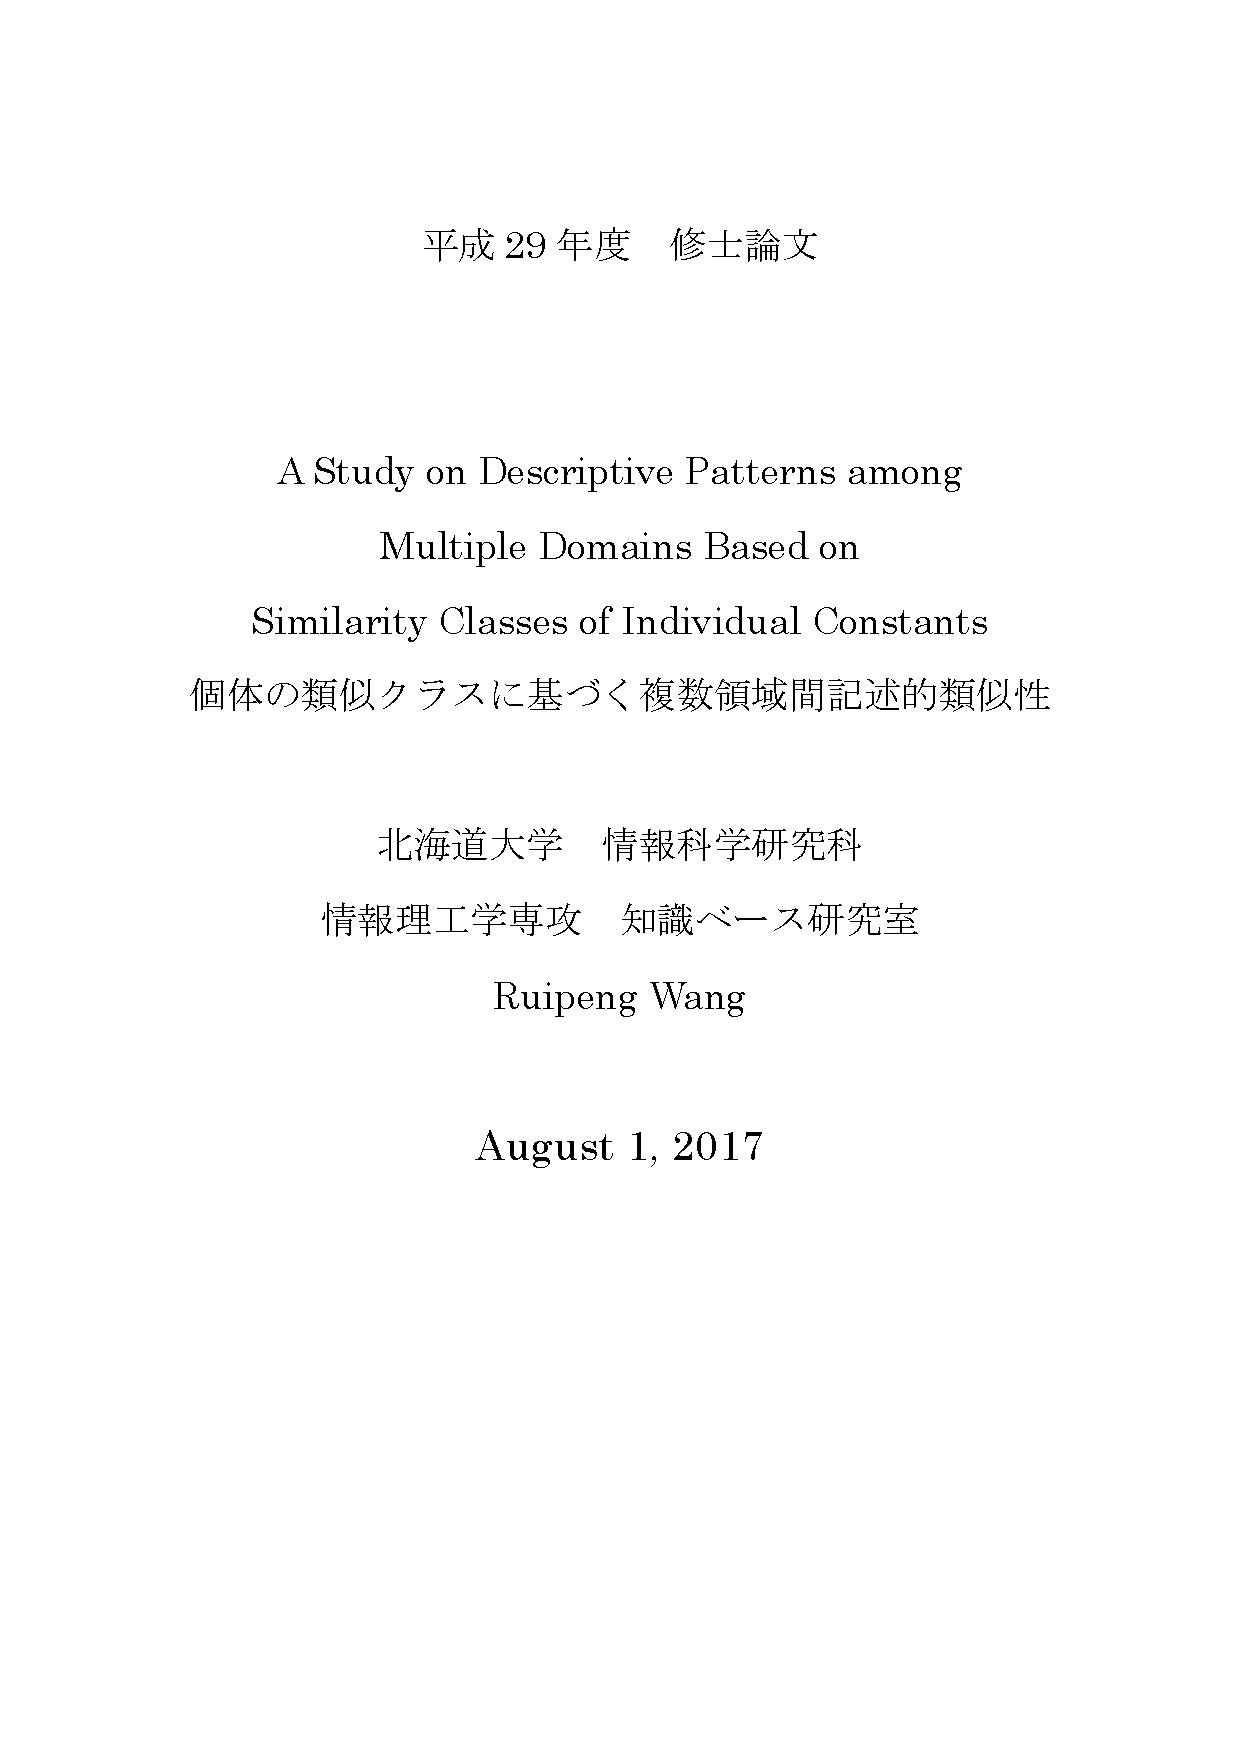
\includepdf{page.pdf}
\newpage


\begin{abstract}
Law plays a very important role in our humans' lives, at the present time, People always would like to use the law to protect their rights. Although we know old precedents is very helpful for new cases, there is also a fact that precedents are very long and very difficult to understand for our laymen. It is also not an easy work for specialists to find similar points among numbers of old precedents in a short time. In this paper, we proposed a method to extract similar parts of different precedents using the concept of descriptive patterns among multiple domains based on similarity classes of individual constants.

\end{abstract}

\textbf{\large Keywords: Descriptive Pattern, Data Mining, Formal Concept,Clique, KeyGraph. }
\tableofcontents


\chapter{Introduction}
\section{Background}
We have to say that law plays a very important role in our humans' lives, Law is a system of rules that are created and enforced through social or governmental institutions to regulate behavior.
Law as a system helps regulate and ensure that a community show respect, and equality among themselves. It is a huge system which holds different kinds of aspects such as maintaining equality, punishing the sinner, Coordination of disputes, etc. It is the rule of human society.
\begin{figure}[!h]
\centering
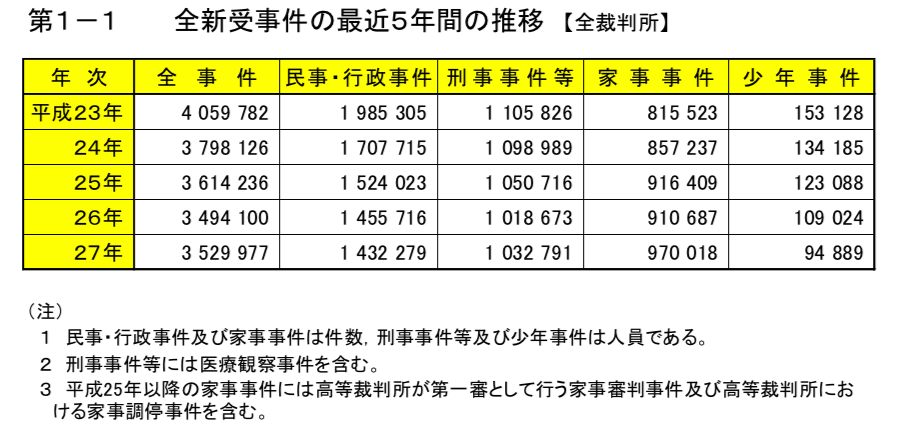
\includegraphics[width=350pt]{./pictures/0101.png}
\caption{information of cases accepted by all courts in Japan}
\end{figure}
\\At the present time, People always would like to use the law to protect their rights, besides civil cases, commercial cases, or even criminal cases. More and more people are dealing with family disputes through legal means. According to the newest data of Court of Japan(Http://www.courts.go.jp)[2], 3529977 new cases have been accepted by different courts, besides local courts, and the supreme court in H.27. The number of family cases accepted is increased by 18.9\% from 815523 cases to 970018 cases during the past five years (data of H.23 to H.27).
\\
Although we know old precedents is very helpful for new cases, there is also a fact that precedents are very long and very difficult to understand for our laymen. It is also not an easy work for specialists to find similar points among numbers of old precedents in a short time.
\\
Hard back to our subject, we want to propose a workable method, which should be easily accessed, highly efficient, to find descriptive similarity points among numbers of precedents.
\begin{figure}[!h]
\centering
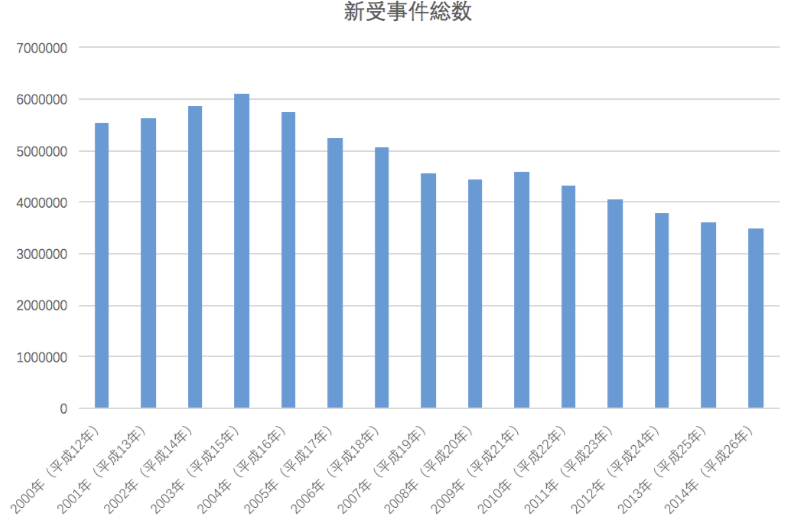
\includegraphics[width=400pt]{./pictures/0101-1.png}
\caption{the number of new litigations in recent years}
\end{figure}
\section{Descriptive Similarity}
There exists a kind of similarity among different articles, although the stories from the different articles are totally discrepant, they may have the same structure of the stories.
\\
\begin{figure}[!hbp]
\centering
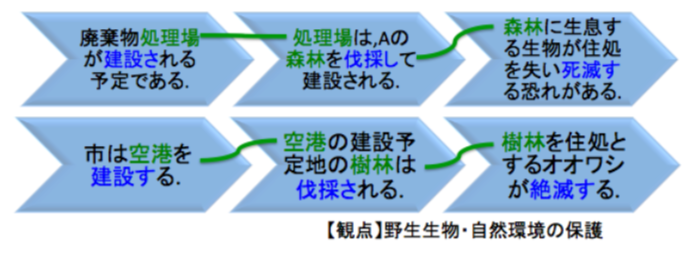
\includegraphics[width=350pt]{./pictures/0102.png}
\caption{descriptive similarity}
\end{figure}
\\
From the example giving in the figure, we can easily understand the descriptive similarity between different articles among the accept of text structure. [10]
\\
Among articles with the descriptive similarity, we can say,
\begin{enumerate}
\item The structure of equivalents is similar.
\item The article contains similar stories.
\end{enumerate}
We call this kind of similarity the descriptive similarity. We would like to extract it among different articles.
Here are two stories to makes is more easy to understand descriptive similarity between different stories.[13]\\ \\
Story 1 
\begin{CJK}{UTF8}{ipxm}
\textbf{あやしい牛}
\end{CJK}
\\ \\ 
\begin{CJK}{UTF8}{ipxm}
昔、福井は夜になっても大勢の人が行き交う、とても栄えた町だった。\\
ところがある夜から、金色の二つの光を持った化け物が現れ、町の八百屋を荒らして回るようになった。怖がった人々は夜に出歩かなくなり、町はだんだんとさびれていった。\\
困った若者たちが、夜の八百屋を見張っていると、化け物の正体はどうやら牛である事が分かった。すると牛飼いと名乗る不思議な老人が現れ、怪しい牛は「どこかの看板から抜け出た牛ではないか」と言う。そこで、町の薬屋の木彫りの牛の看板を確認すると、牛の蹄(ひづめ)にはまだ湿った土が付いていた。\\
彫り物の名人である「左甚五郎」作の立派な木彫りの牛が、夜な夜な看板から抜け出して福井の町を荒らしまわっていたのだった。牛飼いの老人が、看板の牛の両目と前足にノミで傷を入れると、二度と町中に怪しい牛が出没する事も無くなった。\\
それ以来、福井の町は再びにぎわいを取り戻した。その後しばらくして、八幡神社の境内に小さなお堂が建てられ、この牛の看板を大切に奉った。\\
\end{CJK}\\ \\
Story 2 
\begin{CJK}{UTF8}{ipxm}
\textbf{あばれ鹿}
\end{CJK}\\ \\
\begin{CJK}{UTF8}{ipxm}
昔、伊豆は函南村(かんなみむら)の辺りでは、夜な夜な2頭のつがいの大鹿が現れ、田畑を荒らしまわるので、村人は大層困っていた。そこで村人は、猟師の勘七(かんしち)に大鹿を退治してくれるよう頼んだ。\\
勘七は火縄銃を持つと、猟犬とともに狩野川(かのがわ)の川べりにやってきた。そこで夜が来るのを待ち、大鹿を待ち伏せようというのだ。\\
さて、夜になると、勘七が思ったとおり2頭の夫婦(めおと)の大鹿が手前の畑に現れた。勘七は、大鹿を火縄銃が撃てる所まで引き付けるため、猟犬を大鹿の後ろからけしかけた。猟犬にけしかけられた大鹿は、勘七の目論見どおり勘七の前に走って来る。\\
ところが、2頭の大鹿は勘七の目の前で大きく飛び跳ねたのだ。勘七は不意を突かれたものの、かろうじて雄鹿を撃つことが出来た。しかし、勘七の放った弾は確かに雄鹿に命中したのだが、不思議なことに雄鹿の姿はどこにも見当らなかった。\\
夜が明けてから勘七が辺りを見回すと、2頭の鹿の足跡が村の方へと続いている。勘七が足跡を追うと、それは興聖寺(こうしょうじ)の境内で途切れていた。勘七が住職に事情を話し、寺の本堂を調べていると、勘七の猟犬は住職の寝室の方に向かって吠えている。勘七が寝室を開けると、そこには見事な夫婦の鹿の襖絵(ふすまえ)があった。勘七が近づいて見てみれば、なんと雄鹿の胸には勘七に鉄砲で撃たれた傷があるではないか。\\
この大鹿の襖絵は、さる高名な絵師によって描かれたもので、その出来栄えがあまりに見事だったゆえ、ふすまの中から大鹿が現れ出たのだった。しかしこの夫婦の大鹿、勘七に鉄砲で撃たれてからは、恐れをなしたのか、襖の中から出て来ることは二度となかったそうだ。\\
\end{CJK}\\
These pair of stories come from different provinces in Japan. While they seem to be talking about the different things that happen in completely different palaces, but we can easily see that all the stories have a similar process: wired animals come out from some places, destroys the crop and affects the people's life. With the help of capable people, the animals return to their original place and the country isin harmony again.
So far we have introduced the definition of descriptive similarity and gave an example of it. Our research is to extract descriptive pattern base on descriptive similarity.
\section{Previous Work}
Some Research has been done before, the study of this thesis comes after some seniors' effort. For example, Ryo Kita's research ``Matching Legal Aspects with Cases based on Descriptive Similarities'' and Zhang Xiaolong's research ``Towards a Detection of Descriptive Similarities among Multiple Precedents Based on Formal Concept Analysis''. Some important points are used for reference such as the using of KNP tool, the similarity between noun-object similarity classes, using the database of legal precedents, etc. There are still very different points between the seniors' research and this research.
In Ryo Kita's research, the event is a verb and noun pair, think of the matching as a transmission problem the matching is one on one between the abstract and main text of a precedent.[12]\\
In Zhang Xiaolong's research, the event is defined as a list of the verb and noun pairs, this point is the same as this thesis. In his research, he regards the events of each precedent as a concrete graph, and try to find the similar structure of the concrete graphs and build the similar structure as an abstract graph. He also only concerns the matching between two documents.[13]\\
\begin{figure}[!hbp]
\centering
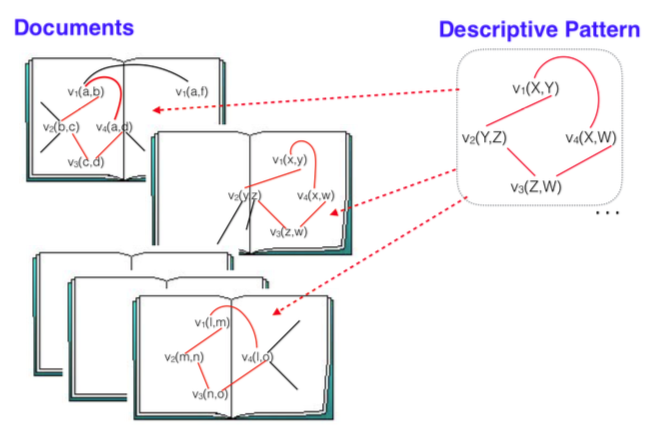
\includegraphics[width=300pt]{./pictures/0103.png}
\caption{Zhang's research}
\end{figure}
Both of them uses the importance of noun defined by the KeyGraph algorithm, but they didn't verify the result of KeyGraph, how the High KeyScore nouns influence the result of similarity classes, we will use some sections to talk about the result of KeyGraph, and whether is it safe to disregard nouns which are not high KeyScore nouns.\\
Besides, we don't concern the event graphs, we proposed a method to extract descriptive patterns from maximal closures.\\
We have three new points to experiment as they are very important points:
\begin{enumerate}
\item We don't use the idea of the concrete graph and abstract graph, although they exist as a fact, we use a more direct way to extract descriptive patterns.
\item We concern more than two documents, the problem will be not a matching problem, it becomes a kind of data mining problem.
\item We will verify the feasibility of KeyGrpah, and talk about the result of it.
\end{enumerate}
\section{Multi-document Summarization}
A multi-document summarization is an automated program designed to extract information from multiple texts of the same subject. The resulting summary report allows individual users such as professional information consumers to quickly become familiar with the information in a large number of document sets. In this way, the multi-document summary system is supplementing the next step to process the information overloaded news aggregator.\\
The information report of Multi-document summarization created is both concise and comprehensive. Putting different opinions together and summarizing, each topic is described from multiple perspectives in a single document. While the goal of a brief summary is to simplify information search and cut the time by pointing to the most relevant source documents, the comprehensive multi-document summary should itself contain the required information, hence limiting the need for accessing original files to cases when refinement is required. The automatic summary provides information that is extracted from multiple sources without any editorial touch or subjective intervention, making it completely unbiased.\\
Because the result of Multi-document summarization is one brief summary, it becomes a little different from our research. For a set of document, there exist a lot of descriptive patterns depend on the complexity of the document set. We can only extract some major ones from them, hence our research becomes a kind of data mining problem. We can also extract some similar point from some very different documents. That is very different with Multi-document summarization.\\ 
\section{Overview}
In this paper, we have five parts, in Chapter 1, we have introduced our background and aim, and the basis of our research, the descriptive similarity.
\\
In Chapter 2, we will introduce some tools we used in our research, such as the precedent database, KNP system, and some import algorithm we need to use in our search, for example, KeyGraph and CLIQUES.
\\
Chapter 3 will contain some important definition of our search and the main algorithm based on our experiment. We will discuss the result and evaluation of the experiment in Chapter 4.
\\
Finally, in Chapter 5, we will summarize our research we have done and some the problem we have met during the experiment. We also have some idea to improve our research in the future.
\chapter{Prerequisite Knowledge}
\section{Precedent}
Japanese new constitution started from 1947. The re-establishment of the whole legal system also began in 1947 to conform to the new constitutional principles. The Constitution in the three basic characteristics features. First, it transplants from US customary law system. Second, it overthrew the emperor of the divine monarchy, established a guarantee for modern civil liberties, in accordance with the principles of democracy legal system. Third, article ninth of the constitution to renounce war and military, to become the ``peace constitution''.\\
Under the Japanese civil law system, court cases provide the criteria for how the law should be interpreted in reality. Although without judicial restraint, the judge also seriously considers the case, especially the Supreme Court's decision, which makes the understanding of precedent become the basis of the implementation of the law.\\
In our research, we use a precedent database provided by D1-Law[3], DAI-ICHI HOKI co., Ltd. This database is contracted with Hokkaido University and can be accessed from within the university network. In addition, ``Court case information'' on the court website, provided by Westlaw Japan Co. There is an available database such as ``Japanese law general online service'', Supreme Court judicial precedent explanation and others. In each case, it is possible to search using case number, incident name, trial judgment date, etc. Considering the number of judicial cases, ease of access, search function, etc. In our research, we decided to use ``D1law.com.'' There are some features of the database.
\begin{enumerate}
\item Japanese largest precedent database with over 210,000 precedents and over 29000 legal provisions.
\item Advantage search supported by the database, we can easily search precedents from the point of legal provisions.
\end{enumerate}
In D1-Law database, we can find some important information of each precedent: 
\begin{enumerate}
\item Basic Information: Precedent ID, Date, Results, etc. 
\item Precedent Main Text: the explanation of the case includes Main Text, and Facts and Reasons.
\item Precedent Abstract: a summarization by the specialist from legal provision view. 
\end{enumerate}
The Precedent Main Text part is the main part of a case. The part Main Text is a part of a brief description of the case. The part Facts and Reasons contains long text and detailed description.\\
The part Facts and Reasons is not a specific configuration required in a case. According to an unwritten customary, almost all precedents have this part as a fact. This part contains four kinds of information: Claim, Indisputable fact, Dispute and Propositions, and Court decision.\\
In our research, we mainly use Precedent Main Text as documents to study descriptive similarity among them.\\
Here is a part of list of the precedents we used in our research(20 of 100).\\
\newpage
\begin{table}[!h]
\centering
\begin{tabular}{ccc}
\hline
Serial number&Precedent ID&Precedent Name\\
001&25000036&\begin{CJK}{UTF8}{ipxm}損害賠償請求上告事件\end{CJK}\\
002&25000038&\begin{CJK}{UTF8}{ipxm}木曽駒高原眺望権訴訟\end{CJK}\\
003&35000044&\begin{CJK}{UTF8}{ipxm}釧路違法公正証書損害賠償請求訴訟\end{CJK}\\
004&27805492&\begin{CJK}{UTF8}{ipxm}国家賠償請求事件\end{CJK}\\
005&27807602&\begin{CJK}{UTF8}{ipxm}中和歌山観音竹商法損害賠償請求訴訟\end{CJK}\\
006&27807603&\begin{CJK}{UTF8}{ipxm}損害賠償請求事件\end{CJK}\\
007&27807929&\begin{CJK}{UTF8}{ipxm}沼津セクシュアル・ハラスメント訴訟\end{CJK}\\
008&27809649&\begin{CJK}{UTF8}{ipxm}損害賠償請求事件\end{CJK}\\
009&27811304&\begin{CJK}{UTF8}{ipxm}損害賠償請求控訴事件\end{CJK}\\
010&27811611&\begin{CJK}{UTF8}{ipxm}損害賠償請求事件\end{CJK}\\
011&27813101&\begin{CJK}{UTF8}{ipxm}日鉄鉱業松尾採石所じん肺訴訟控訴\end{CJK}\\
012&27814650&\begin{CJK}{UTF8}{ipxm}損害賠償請求控訴事件\end{CJK}\\
013&27816661&\begin{CJK}{UTF8}{ipxm}東京電力(群馬)事件\end{CJK}\\
014&27816925&\begin{CJK}{UTF8}{ipxm}損害賠償請求事件\end{CJK}\\
015&27818787&\begin{CJK}{UTF8}{ipxm}損害賠償請求事件\end{CJK}\\
016&27818788&\begin{CJK}{UTF8}{ipxm}勧角証券違法勧誘損害賠償請求事件\end{CJK}\\
017&27818866&\begin{CJK}{UTF8}{ipxm}損害賠償請求事件\end{CJK}\\
018&27820817&\begin{CJK}{UTF8}{ipxm}東京電力事件(山梨東電訴訟)\end{CJK}\\
019&27824746&\begin{CJK}{UTF8}{ipxm}損害賠償請求事件\end{CJK}\\
020&27825841&\begin{CJK}{UTF8}{ipxm}債務不存在確認請求-同反訴請求事件\end{CJK}\\
\hline
\end{tabular}
\end{table}
\section{KNP tool}
KNP tool is a system which can perform parsing, case and anaphora analysis in Japanese texts.[4] It is provided by Kurohashi-Kawahara Laboratory of Kyoto University. It can use the parsing result of JUMAN system as the input and get dependency relationship, anaphora relationships, etc. It bases on a probability model which is automatically generated from the Web. In our research, We use KNP tool to extract the dependency case relationships between nouns and verbs. It lasts very long to analysis a long text, we need to divide the documents into short ones, or even sentences for a correct result. All of these have been done before our experiment. \\
After inputting a Japanese sentence, we can get a verb and the nouns that according to it. Verb, and nouns according to it, is the basis element of our research. We have a name of Event for it, we will have a detailed introduction in later Chapter. Here is a simple example of KNP result.\\
\begin{figure}[!h]
\centering
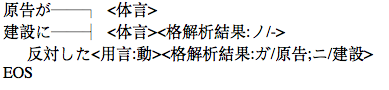
\includegraphics[width=250pt]{./pictures/0202.png}
\caption{a result of KNP tool}
\end{figure}
In our example, the original sentence is \begin{CJK}{UTF8}{ipxm}`原告が建設に反対した.'\end{CJK}, We can find that, in this sentence, the verb is \begin{CJK}{UTF8}{ipxm}`反対する'\end{CJK}, nouns are \begin{CJK}{UTF8}{ipxm}`原告'\end{CJK} and \begin{CJK}{UTF8}{ipxm}`建設'\end{CJK}, especially, \begin{CJK}{UTF8}{ipxm}`原告'\end{CJK} is in \begin{CJK}{UTF8}{ipxm}`が case'\end{CJK}, and \begin{CJK}{UTF8}{ipxm}`建設'\end{CJK} is in \begin{CJK}{UTF8}{ipxm}`に case'\end{CJK}. There are over 20 kinds of cases that can be extracted by KNP tool, in our research, we use some important ones, they are \begin{CJK}{UTF8}{ipxm}`ガ', `ヲ', `ニ', `ト', `デ', `カラ', `ヨリ', `マデ', `ヘ' and `時間'\end{CJK}. Because KNP comes from a big data from Web and uses a probability model, the correctness can be ensured. But KNP tool does nothing with passive sentences, We have to hand them by ourselves, for example, \\
\begin{CJK}{UTF8}{ipxm}  
`原告は被告を訴えた.'
\end{CJK}\\
\begin{CJK}{UTF8}{ipxm}
\CJKtilde  
`被告が原告に訴えられた.'
\end{CJK}
have the same meaning, but the cases of the nouns are totally different. We will have a transfer for passive sentences: 
\begin{enumerate}
\item \begin{CJK}{UTF8}{ipxm}`が case' to `よ case'\end{CJK}
\item \begin{CJK}{UTF8}{ipxm}`に case' to `が case'\end{CJK}
\item \begin{CJK}{UTF8}{ipxm}`による case' to `が case'\end{CJK}
\end{enumerate}
Although KNP is a very powerful tool, the result of KNP tool contains kinds of information. It is very hard for everyone to understand the result of KNP, and here I give an example to show how to read the output of KNP tool.\\ \\
\newpage
\textbf{Example of KNP}\\ \\
Input:\begin{CJK}{UTF8}{ipxm}麻生太郎はコーヒーを買って飲んだ。\end{CJK}\\
Option: -simple -anaphora\\
Output:\\
\begin{figure}[!h]
\centering
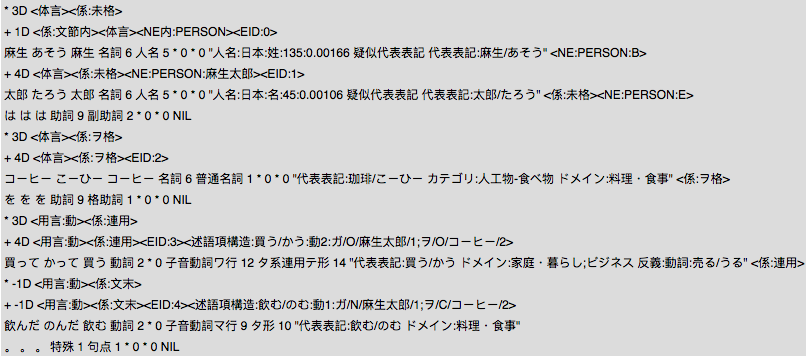
\includegraphics[width=350pt]{./pictures/0202-1.png}
\caption{example of KNP output}
\end{figure}
\\
Line starts with `$*$':
\begin{enumerate}
\item Information on clauses
\item In the case of the example in the example, the line beginning with "* 3D" at the head is ``Aso Taro'' (clause number = 0), the line beginning with ``* -1 D'' corresponds to``drunk'' (clause number = 3) 
\item The first digit represents the clause number (since the sentence at the end of the sentence does not have an affiliation, it is always output as ``-1'')
\item The following alphabet represents the type of dependency, and it is output as D for normal dependency relations, P for parallel etc.
\end{enumerate}
Line starts with `$+$'
\begin{enumerate}
\item Information on basic phrases
\item In KNP, basically it deals with dependency in the unit called "basic phrase consisting of one independent word and its adjunct
\item In terms of clause units ``Aso Tar'' becomes one clause, but when considered in basic phrase units, ``Aso'' and ``Taro'' are the two basic phrases
\item Forms such as dependency are the same as those starting with *
\end{enumerate}
After this transformation, almost all passive sentence can be correctly handled. From the detailed result of KNP, we can know whether a sentence is an active one or a passive one. Therefore, we can apply this transformation to convert our results.\\
KNP result will be our original data for our experiment.
\section{KeyGraph Algorithm}
Extracting keywords from a document is not an easy task with normal tools[9], we use Keygraph Algorithm to solve the problem. In Keygraph, we extract keywords representing the asserted main point in a document, without relying on external devices such as natural language processing tools or a document corpus. It is based on Graph Segmentation, representing co-occurrence relationships among terms in the document, forming clusters. Each cluster corresponds to the concepts that the author's ideas are based on, and the top terms are chosen as keywords based on the statistics of each word's relation to these clusters. Because it only uses the idea of graph and statistic, it works very fast to extract keywords.\\
To build a building, we need a foundation. And the walls, the doors and windows, and all kinds of decorations. However, the nature of the building is to protect the inhabitants from solar radiation and Rainstorm on the roof. To support the roof, we need some more columns.\\
Similarly, to write a good document, we first need to know that the basic concept of the document is based on the first step. The detailed description needed to configure documents, metaphors, and samples is also essential. Last but not least, in order to emphasize the main points, such as the column of a building, it is also necessary to deploy content in the document.\\
Keygraph uses the idea of building, and have the features as follow[5]:
\begin{enumerate}
\item expressing the main point of the author, not frequent terms.
\item using only information in the text of documents without NLP tools.
\item working very fast.
\end{enumerate}
There are three steps to achieve the algorithm.
\begin{enumerate}
\item extracting foundations: basic and preparatory concepts are obtained as clusters base on the co-occurrence nouns.
\item extracting columns: the relationships between nouns and concepts are obtained.
\item extracting roofs and keywords: nodes at the cross of strong columns.
\end{enumerate}
When we have a document, we call it $D$, is composed of sentences, which are in turn composed of words.\\
Beforehand, we have a noise list of non-significant words, which have less meaning. We call it stop words list and it contains words such as `a', `and', `here', etc. We also need to transform words to original form, for example, `do', `doing', and `does', are same words, we need to reduce them all to `do'. Then our $D$ is represented by $D_{terms}$ include unique terms, $D_{terms} = \{w_1, w_2, w_3,...\}$, each term is a word or a phrase in $D_{terms}$. Then we can start our algorithm.[5]\\ \\
\textbf{Extracting\ Foundations}\\ \\
We need to make a Graph $G$ for document $D$, which is made of nodes representing terms, and the links representing the co-occurrence. First, the nodes are high-frequency terms in $D$, and they become the candidates of the foundation. We choose the top-30 high-frequency terms as nodes and, we call them $HF$. That means terms in $HF$ become terms in $G$. We link the nodes in $HF$ if their association is strong, here, we define the association of terms $w_i$, and $w_j$ in $D$, as
\begin{displaymath}
assoc(w_i,w_j) = \sum_{s \in \mathcal{D}} min(|w_i|_s, |w_j|_s),
\end{displaymath}
where $|x|_s$ means the count of $x$ in sentence $s$. After that, we have built our foundations. It doesn't matter whether $G$ is a connected graph or not. We call the connected ones, clusters.
\begin{figure}[!hbp]
\centering
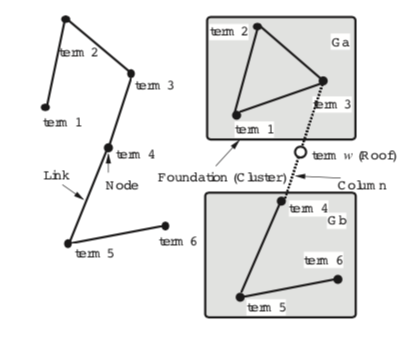
\includegraphics[width=250pt]{./pictures/0203.png}
\caption{Extracted foundations as $G_a$ and $G_b$}
\end{figure}
\\ \\
\textbf{Extracting\ Columns}\\ \\
Keywords that we want are important terms that can hold all the clusters. We assign value $key(w)$ for each term $w$ in document $D$. $key(w)$ in a number between 0 and 1, which is defined as the probability of term $w$ to appear if all the foundations in $G$ are considered. We have defined $|x|_s$ as the count of term $x$ in sentence $s$, we also have $|g|_s$, which is the count of cluster $g$ in sentence $s$, as the count of terms in $s\cap g$. We define based and neighbors as,
\begin{displaymath}
based(w,g) = \sum_{s \in \mathcal{D}}|w|_s|g-w|_s
\end{displaymath}
\begin{displaymath}
neighbors(g) = \sum_{s\in \mathcal{D}}\sum_{w\in s}|w|_s|g-w|_s
\end{displaymath}
where,
\begin{displaymath}
|g-w|_s = |g|_s - |w|_s,\ if \ w \in g
\end{displaymath}
$based(w,g)$ is the co-occurrence degree between term $w$ and other terms in cluster $g$. $neighbor(g)$ is the count of terms in sentences including terms in $g$.\\
base on these functions, $key(w)$ is defined as follow,
\begin{displaymath}
key(w)=1-\prod_{g\in \mathcal{G}}(1-base(w,g)/neighbors(g))
\end{displaymath}
That means,
\begin{displaymath}
key(w) = probability(w|\bigcap_{g \subset \mathcal{G}}g)
\end{displaymath}
or it is logically equivalent to that,
\begin{displaymath}
key(w) = probability(\bigcup_{g\subset \mathcal{G}}(w|g))
\end{displaymath}
Sorting all the terms in $D$ by keys produces a list of terms ranked by their association with the clusters. We choose top-12 key terms as high key terms.\\ \\
\textbf{Extracting\ Roofs,\ Keyword}\\ \\
After works before, we need to add all the high key terms as new nodes to $G$, of course, if they are not in $G$ yet. The keywords are not high keys, there may exist especially important foundations are of low keys but highly ranked by the sum of the strength of touching columns. We still have some other processing. Column is a value between a high key term $w_i$ and a high-frequency term $w_j$, as
\begin{displaymath}
column(w_i,w_j)=\sum_{s\in \mathcal{D}}min(|w_i|_s,|w_j|_s)
\end{displaymath}
We can sort them by $column(w_i,w_j)$ for columns touching $w_i$, for each high key term $w_i$. columns with highest column values and connecting term from two different clusters are selected to create new links. and finally, we make a keygraph for a document.\\
Nodes in $G$ are sorted by the sum of columns. We choose top-12 terms as the keywords that extracted by KeyGraph Algorithm.
We have realized the algorithm by Python language, in the section after, we will have some experiment on evaluating the result of KeyGraph, Here we have a simple example of KeyGraph on Japanese stories.
\begin{figure}[!hbp]
\centering
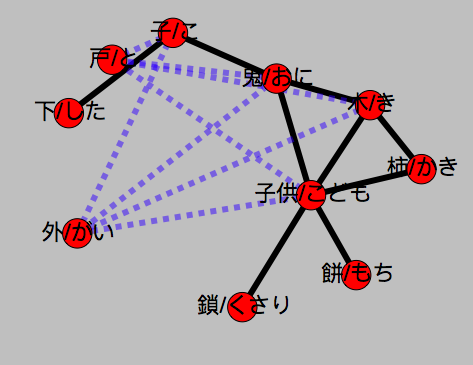
\includegraphics[width=250pt]{./pictures/0203-1.png}
\caption{an example of KeyGraph}
\end{figure}
\section{CLIQUES Algorithm}
In our research, we will use the idea of the clique to extract the candidate of descriptive patterns, to be exact, bipartite clique. In the mathematical field of graph theory, a clique is a subset of the vertices of an undirected graph, so that each of the two vertices of the subgraph is adjacent to each other, that is, its induced subgraph is complete. Cliques are one of the basic concepts of graph theory. They are also widely used in many other mathematical problems and graph theory, it is also very popular in computer science: the task of finding whether there is a clique of a given size is NP-complete. But although the hardness results for many factions, many algorithms have been studied. What we talk here is one of them called CLIQUES, developed by Etsuji Tomita, Akira Tanaka, and Haruhisa Takahashi, from The University of Electro-communications. We can find maximal cliques from a graph by CLIQUES Algorithm, we will talk about how to do with the bipartite graph, and find bipartite cliques.\\
In the mathematical field of graph theory, a bipartite graph is a graph where the vertex in it can be divided into two disjoint sets $U$ and $V$, $U$ and $V$ are each independent sets. And every edge connects one vertex in $U$ and one vertex in $V$. Bipartite Clique is a special subgraph of a bipartite graph, where each pairs from vertex set $U$ and vertex set $V$  are connected. If we connect all vertex form $U$ with each other and do the same process to set $V$, we can find a bipartite clique becomes a normal clique. Conversely, if we want to find bipartite cliques in a bipartite graph, we can connect all vertexes from the same set, and make it be a normal graph, the vertexes in clique also form bipartite clique as a subgraph of the original bipartite graph. We will introduce CLIQUES Algorithm which can extract all maximal cliques form a graph very fast.\\
CLIQUES is a depth-first algorithm for generating all maximal cliques of an undirected graph, in which pruning methods are employed as in the B-K algorithm[8]. All of the results, which are maximal cliques are produced in a tree-like form. And its worst-case time complexity is $O(3^{n/3})$ for an n-vertex graph.[6] \\
We are concerned a simple undirected graph $G=(V,E)$ with a finite set $V$ of verices and a finite set $E$ of unordered pairs $(v,w)$ of idstinct vertices, we call them edges. We also call the pair of vertices $v$ and $w$ adjacent if $(v,w)\in E$. For any vertex $v\in V$, we call $\mathcal{T}(v)$ is the set of verties that are adjacent to $v$ in $G = (V,E)$, For example, $\mathcal{T}(V) = \{w\in V | (v,w)\in E\}$. For a subset $W \subseteq V$ of vertices, $G(W) = (W,E(W))$ with $E(W)=\{(v,w)\in W \times W|(v,w)\in E\}$ is called a subgraph of $G = (V,E)$ induced by $W$. For a set $W$ of vertices, $|W|$ donotes the number of elements in $W$. Given a subset $W \subseteq V$ of vertices, the induced subgraph $G(Q)$ is called to be complete if $(v,w)\in E$ for all of vertices $v,w \in Q$ with $v \ne w$. In this situation, we can simply state that $Q$ is a complete subgraph. We call a complete subgraph a clique. We call a clique a maximal clique if the clique is not a proper subgraph of any other cliques. After understand the basic knowledge about clique, we can start our algorithm.[6]\\ \\
\textbf{CLIQUES}
\\ \\
We have mentioned before, CLIQUES is a depth-first algorithm for generating all maximal clique of a give undirected graph $G=(V,E)\ V\ne \emptyset$.\\
For the processing of algorithm, we have a global variable $Q$ of a set of vertices that constructs a complete subgraph, clique, found up. THe algorithm starts with set $Q$ as an expty set, and expands $Q$ step by step over applying the recuresive procedure $EXPAND$ to $V$ and its goal induced subgraphs to search for all complete subgraphs until they become maximal subgraphs.\\
Let $Q = \{p_1,p_2,...p_j\}$ become a complete subgraph found over some processing, and consider the vertices:
\begin{displaymath}
SUBG = C \cap \mathcal{T}(p_1)\cap \mathcal{T}(p_2)\cap ... \cap\mathcal{T}(p_j)
\end{displaymath}
where $SUBG=V$ and $Q = \emptyset$ as the initialization. We apple $EXPAND$ to $SUBG$ for searching for a larger complete subgraph. If we meet the situation of $SUBG = \emptyset$, we can say $Q$ is a maximal complete subgraph, or a maximal clique. Else, $Q\cup{q}$ will be a larger complete subgraph for every $q\in SUBG$. In this case, we consider a smaller subgraph set $G(SUBG_q)$ in which the graphs are induced by new set of vertices:
\begin{displaymath}
SUBG_q = SUBG \cap \mathcal{T}(q)
\end{displaymath}
for all $q \in SUBG$; we will also apply $EXPAND$ to $SUBG_q$ for finding larger complete subgraphs containing $Q\cup{q}$.\\
So far, we have only described the well-known basic framework of generating algorithms for all the maximal complete subgraphs, maximal cliques. This process can be represented by the following search or collection of search trees: The root set of the search forest is exactly the same as the $V$ of the graph $G = (V, E)$. For each $q \in SUBG$, all vertices in $SUBG_q$ are children of q. Thus, a set of vertices along the path from the root to any vertex of the search tree form a complete subgraph or we can say a clique.\\
The most important point of CLIQUES Algorithm is pruning unnecessary parts. We have two methods, which are the same as the Brom-Kerbosch Algorithm.We treat the previously constructed $SUBG(\ne \emptyset)$ as an ordered set of vertices, and we continue to generate maximal cliques from the vertices in the SUBG in order.\\
First of all, $FINI$ will be the sebset of vertices of $SUBG$ which have benn processed by the algorithm. We use $CAND$ to represent the remaining sets of extended candidates: $CAND = SUBG-FINI$, So we have:
\begin{displaymath}
SUBG = FINI \cup CAND
\end{displaymath}
$FINI = \emptyset$ as the initialization. We will also have:
\begin{displaymath}
SUBG_q = FINI_q \cup CAND_q
\end{displaymath}
where,
\begin{displaymath}
FINI_q = FINI \cap \mathcal{T}(q) and CAND_q = CAND \cap \mathcal{T}(q)
\end{displaymath}
According to the processing, we can find that, only the vertices in $CAND_q$ will be the candidates for expanding the complete subgraph $Q\cup{q}$ for find a larger maximal complete subgraph. After that, all the cliques containing $(Q\cup{q})\cup{r}with r\in FINI_q \subseteq FINI$ will generate for any $r$ by the processing of procedure $EXPAND$ to $FINI$.\\
The second step, Given a vertex $u \in SUBG$, it is assumed that all the maximal cliques containing $Q \cup {u}$ have been generated. Then each new maximal clique containing $Q$ instead of $Q \cup {u}$ must contain at least one vertex $q \in SUBG - (u)$. This is because $R \cup {u}$ is a larger complete subgraph if $Q$ is extended to a complete subgraph $R = (Q\cup S) \cap (SUBG - {u})$ with $S \subseteq SUBG \cap (u)$ So $R$ is not a maximal one. Thus, by extending $Q$ to $Q \cup {q}$, any new largest group can be found such that $q \in SUBG - (u)$, and then all sets containing $Q \cup {q}$ are generated.\\
\newpage
From the following figure, we can easily understand the processing of CLIQUES Algorithm.
\begin{figure}[!hbp]
\centering
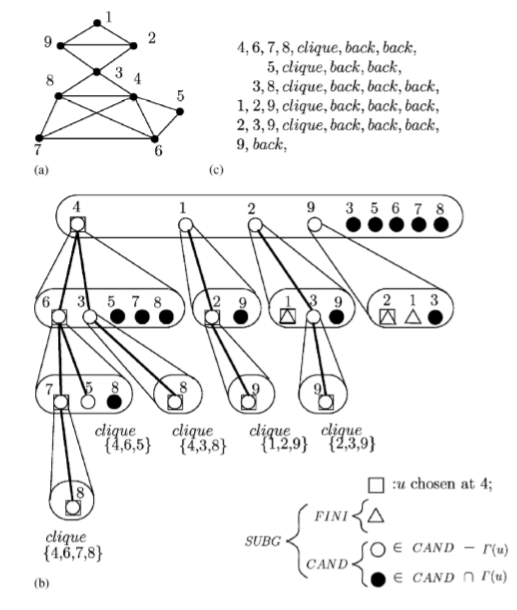
\includegraphics[width=400pt]{./pictures/0204.png}
\caption{an example of CLIQUES Algorithm}
\end{figure}
\newpage
In our research, we won't use any normal maximal, we will use the bipartite maximal cliques. To get bipartite maximal cliques from the bipartite graph using CLIQUES algorithm, we need some techniques. We have a figure to show it clearly.
\begin{figure}[!h]
\centering
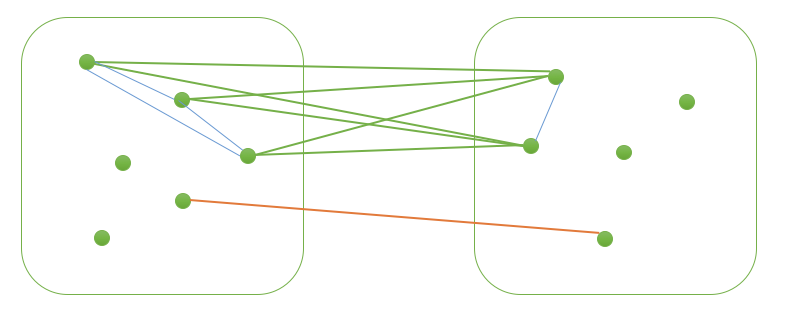
\includegraphics[width=350pt]{./pictures/0204-1.png}
\caption{bipartite clique}
\end{figure}
From the figure we can see that, the nodes connected by green link make a bipartite clique, if we also connect all the nodes in the same node set, the bipartite clique becomes a clique. So when we want to find maximal bipartite clique from a bipartite graph, we can connect all the nodes in the same node set, and make a normal graph[7], find the maximal clique in it, we can reconstruct all maximal bipartite clique from the clique result.
\section{Beam Search}
Beam Search is a heuristic graph search algorithm, usually used in the case of very large solution space, in order to reduce the space occupied by the search space and time, in each step of the depth of the expansion, cut off some of the poor quality of the node, keep some of the higher quality of the node. This reduces the space consumption and improves the efficiency of time, but the disadvantage is that there may be potential best solutions are discarded, so Beam Search algorithm is not complete.\\
Beam Search uses a breadth-first strategy to create a search tree that sorts the nodes at the heuristic cost at each level of the tree, and then leaves only nodes of a predetermined number (Beam Width) The node continues to expand at the next level, and the other nodes are cut off. If the beam width is infinite, then the search is the width of the first search. But the disadvantage of the pruning is that there may be some results that potential to be the best solution are discarded in the process above.Thus, the beam search algorithm is incomplete and uninfected. It is usually used in some large systems, such as machine translation systems, voice recognition systems, which can be very large and the only correct solution does not exist. The goal of this system is to use the fastest way to find the most appropriate solution.\\
As we have introduced before, beam search algorithm is a simplified method of the breadth-first algorithm. It has a heuristic function $h$ and a pre-set beam width $B$.\\
The heuristic function h is used to estimate the consumption from the given node to the target node, and the beam width $B$ is responsible for limiting the number of nodes that should be stored in each level of the breadth-first search. That is, the heuristic function allows the algorithm to select the node that directs it to the target node, and the beam width only allows the algorithm to store the important nodes in the memory and prevent it from being exhausted from the memory before finding the target node.\\
The processing is as follow.\\
\begin{enumerate}
\item Insert the initial node into the list,
\item The node will be heap if the node is the target node, the algorithm ends;
\item Otherwise expand the node, take the beam width of the node into the heap. Then go to the second step to continue the cycle.
\item The end of the algorithm is to find the optimal solution or the heap is empty.
\end{enumerate}
The beam width can be pre-set or changed, and you can search by a minimum beam width. If you do not find the appropriate solution, then expand the beam width and find it again.\\
Personally think that the beam search method, in fact, provides a way to find the best solution, that is, in the appropriate circumstances, you can cut some of the low credibility of the path, in actual use, you can each layer of the beam width is inconsistent, For example, in some of the initial level to retain some of the results, in the back can be assured that bold pruning. Of course, you can also live and use, you can combine the depth of priority algorithm, through backtracking, you can find the optimal solution.
\chapter{Proposed Method}
\section{Intorduction}
First of all, we can see a basic idea of our research from Figure. \\
\begin{figure}[!hbp]
\centering
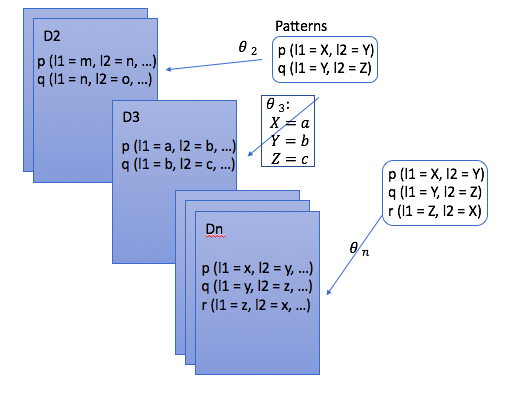
\includegraphics[width=250pt]{./pictures/0301.png}
\caption{Image of extracting descriptive patterns from document set}
\end{figure}
\\
Structural similarity is a kind of similarity that can be explained by a pattern having a special structure, for example, it includes similarity of graphs. We want to find out a descriptive pattern that can be embedded into some event graphs of the precedents. We can think that it is one kind of evaluation of the distance of graphs, it becomes a problem of data mining. To extract descriptive patterns, we need to extract all candidates first. And the re-construct of the descriptive pattern will be a difficult task.\\
In the following sections, we will discuss our idea and a specific algorithm to re-construct the descriptive patterns. In Section 2, we will talk about some basic definitions, which are very useful for our research. In Section 3, we will introduce what the Descriptive Pattern is. Then we will talk about the importance of nouns and cases. Finally, in Section 6, we will propose an idea to re-construct the Descriptive Pattern.
\section{Domains, Events and Patterns}
Let's start with some basic definition. As we have introduced KNP tools in former Chapter, we can extract verbs and nouns in different cases from different sentences. We can define event as this,[1]
\begin{definition}
Given a sentence, we can construct an event $e$ for it, with the predicate and nouns of this sentence:
\begin{displaymath} 
e = p(l_1 = a_1, l_2 = a_2,...l_n = a_n)
\end{displaymath}
where $p$ is the predicate(verb) of a sentence, $a_j$ is a noun, we call it constant symbol, $l_j$ is a case. we can say that 
$a_j = e.l_j$
\end{definition}
After that, we can define the domain,[1]
\begin{definition}
$D_i$ is a set of events. and $const(D_i)$ is a set of const(nouns) in $D_i$. For our data set, we have $D = \{D_1,D_2,...,D_n\}$, we assume that, 
\begin{displaymath}
const(D_i)\cap const(D_j) = \emptyset, \ i\ne j
\end{displaymath}
\end{definition}
For the whole data set, we will also have,
\begin{displaymath}
const(\mathcal{D}) = \bigcup_{i =1}^{N}const(D)
\end{displaymath}
Those are our events and constant set. If we change our nouns t0 abstract variables, we can get abstruct event,[1]
\begin{definition}
Given an event $e'$, use abstract variables to represent the constants,
\begin{displaymath}
e = p(l_1 = X_1, l_2= X_2,...,l_n = X_n)
\end{displaymath}
where $X_j$ is abstruct variables for nouns.
\end{definition}
With the several abstruct events, we can build Pattern as a set of abstruct events.[1]
\begin{definition}
Given a pattern $P$ is the set of abstract events,
\begin{displaymath}
P = {...,e_j,... = p(l_1 = X_1, l_2 = X_2,...,l_n = X_n,...)}
\end{displaymath}
where in each $e$, $l_i \ne l_j$ if $i\ne j$
\end{definition}
We can easily get Domain $D$ from pattern $P$, if we set 
\begin{displaymath}
\theta = {X_1 = a_1, X_2 = a_2,...,X_n = a_n}
\end{displaymath}
We have a support relationship between pattern $P$ and domain $D$: $\preceq$
\begin{definition}
Given a pattern $P$, and a domain $D$, we have support relationship between them if they meet the requirement
\begin{displaymath}
D\preceq P \iff \exists \theta \forall e = p(cl)\in P \exists p(cl_c)\in D \ s.t. \ cl\theta \subseteq cl_c
\end{displaymath}
\end{definition}
for example, domain $D={p(l_1 = a,l_2 = a,l_3 = b),\ q(l_1 = b)} $and pattern $P={p(l_1 = X,l_2=X)}$, meet the condition of $D\prec P$ with $\theta = {X = a}$.[1]
\begin{definition}
Given patterns, there are ordering relationship between them, for pattern $P_s$ and $P_g$:
\begin{displaymath}
P_s \preceq P_g \iff \exists \theta \ s.t. \ (e = p(cl_g)\in P_g \Rightarrow \exists p(cl_s)\in P_s\  with\ cl_g\theta \subseteq cl_s)
\end{displaymath}
\end{definition}
if $P_s\preceq P_g$ and $P_g\preceq P_s$, we can say $P_s \sim P_g$.[1]
\begin{definition}
For $P_s$ and $P_g$, meet the condition of  $P_s\preceq P_g$,and $P_1 \ne P_2$, that means $P_s\prec P_g$ we defin more sepcific as,
\begin{displaymath}
P_s\prec P_g \iff P_s\ more\ specific\ than\ P_g 
\end{displaymath}
\end{definition}
When we have a domain base $\mathcal{D}$ contains a lot of domains,[1]
\begin{definition}
Given a pattern $P$ and a domain base $\mathcal{D}$
\begin{displaymath}
[P] = \{D\in \mathcal{D}| D\preceq P\}
\end{displaymath}
the domains that supported by P[1].
\end{definition}
This is a weak support relationship, we also have a strong relationship, it uses the idea of KeyGraph, we will introduce it in next section.
we say that $P$ is $\tau-supported$ by a case base $D$ if $|[P]|\geq N_\tau$, where $0<t<1$ is a minimum support parameter.we call it minsup condition.
There is a fact that, the relationship meet the condition of monotonicity:
for patterns P and Q,
\begin{displaymath}
P \preceq Q \Rightarrow [P]\subseteq [Q]
\end{displaymath}
\section{Descriptive Pattern}
After the definition of Domains, Events, and Patterns, and the ordering relationship between them, it comes possible to understand the definition of Descriptive Pattern(DP).\\
DP is a minimum pattern among those t-support by D.[1]
\begin{definition}
Given a pattern P, if P meets two requirments:\\
P is $\tau$ -supported. 
\begin{displaymath}
|[P]|\geq N_\tau
\end{displaymath}
P is a minimum(most specific) pattern
\begin{displaymath}
\forall P' \in \mathcal{P}|P' \ne P, s.t.P < P'
\end{displaymath}
We call $P$ is a Descriptive Pattern $DP$.
\end{definition}
We have an example to understand the relationship between Patterns and Domains:
\begin{figure}[!h]
\centering
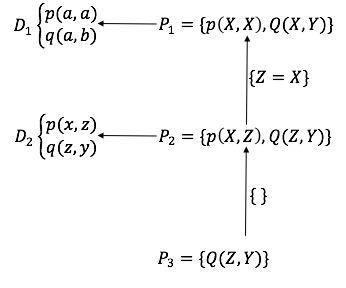
\includegraphics[width=250pt]{./pictures/0303.png}
\caption{Relationship between Patterns and Domains }
\end{figure}
\newpage
From the example, we can see that the variables carry two kinds of information: roles and their fillers:
for example, $P_2$'s $X$ here plays the $l_1 -role$ of $p$, $p(l_1)$.
\begin{table}[!h]
\centering
\begin{tabular}{ccc}
\hline
vars in $P_2$ & role & filler\\
\hline
X & $p(l_1)$ & $a \in D_1$, $x \in D_2$\\
Z & $p(l_2),q(l_1)$ & $a \in D_1$,$z \in D_2$\\
Y & $q(l_2)$ & $b \in D_1$,$y \in D_2$\\
\hline
\end{tabular}
\caption{roles and fillers of variables}
\end{table}
for a pattern P, we can define the role set:[1]
\begin{definition}
Given a variable $X$, and the roles it plays in $\mathcal{D}$,
\begin{displaymath}
role_p (X)={p(l)|p(...,l = X,...) \in P}
\end{displaymath}
is the roles played by $X$.
\end{definition}
$\tau$-supported is the basis condition for patterns to be candidate of $DP$s.\\ \\
\textbf{Least General Generalization}\\ \\
In the initial study of the descriptive pattern, someone have given a method to extract the descriptive pattern from a set of two domains and it can be extended to multi-document situation.
\begin{figure}[!h]
\centering
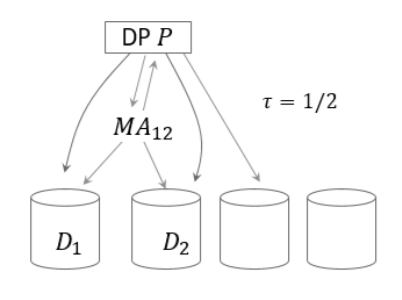
\includegraphics[width=250pt]{./pictures/0303-1.png}
\caption{Least General Generalization}
\end{figure}
That method is called Last General Generalization, LGG.[11] It will generate an indirect value of MA:
\begin{displaymath}
MA_{12} = lgg(D_1,D_2)
\end{displaymath}
From the property of LGG, we will find that $P \preceq MA_{12}$. $MA_{12}$ also meets the the requirment of support $MA_{12}\preceq P$. We can say $P \sim MA_{12}$
From this point,
\begin{displaymath}
DP \iff LGG, LGG\ supported\ by\ N\tau
\end{displaymath}
We can constract DP with LGG with the following method.
\begin{figure}[!h]
\centering
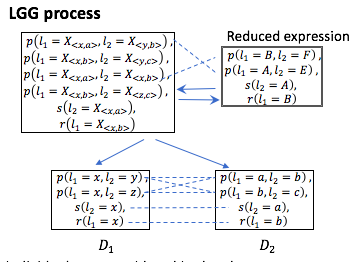
\includegraphics[width=250pt]{./pictures/0303-2.png}
\caption{Least General Generalization}
\end{figure}
For all cases $p(cl)$, we have a sub list of 
$cl_{sub}=\{l_{i_1} = t_{i_1},...,l_{i_n}=t_{i_n}\}$
if we consern 
$p_\{l_{i_1},...,l_{i_n}(t_{i_1},...,t_{i_n})\}$ here, 
$p_l(t)$ 
and $p(l=t)$ have the same meaning. For a event set $Q$, we have $exp(Q)\iff Q$ as all the expend events.
\begin{fact}
$P \preceq D$ by $\theta \iff exp(P)\theta \subseteq exp(D)$
\end{fact}
\begin{definition}
$D_{sel}$: corresponding to $D$ and $\tau$, the set extracted from $N\tau$ domains.
\end{definition}
From that point $lgg(D_{sel})$ is defined as $lgg({exp(D_1),...,exp(D_{N\tau })})$
\\
For a situation of $N\tau > 2$, we will build $N\tau - tuple$ for them as the figure shows,
\begin{figure}[!h]
\centering
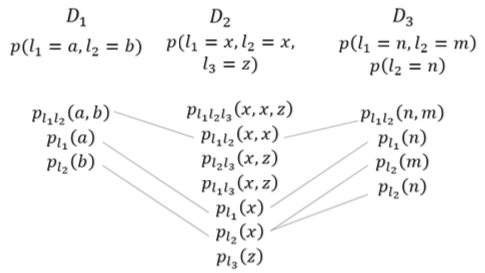
\includegraphics[width=250pt]{./pictures/0303-3.png}
\caption{$N\tau$ = 3 situation}
\end{figure}
For two domains, the pairs of events or individuals are considered in the above construction.
For more than three domains under minimum support parameter less that 1, we need to do consecutive application of LGG or to regard tuples of events/individuals under possible combinations of domains.\\
As the connection of lgg will be increase by square growth.We propose to use neither pairs nor tuples. Similarity classes of individuals over domains: frequent closures (intent of formal concepts)

\section{Importance of Nouns}
The numbers of nouns appear in one document, the amount may be huge depending on the length of the text. From the point of common sense, we have an idea of that, not all nouns are equally significants among the whole text. As we know, for example, `scissors' is much more specific than `tool', In some cases, `scissors' can express a clear and certain meaning. So we can say `scissors' is more important than `tool' in this kind of situation. \\
So, we use KeyGraph algorithm we have introduced before to help us find the most important noun from a document text. Frequency is also very important in determining the importance of nouns.\\
According to the idea of the author, the importance of nouns becomes very different in the different specific document. We can't regard the nouns as the same in a different situation. We apply KeyGraph algorithm to strengthen our support relationship,\\
$D$ supports $P$ if $D \preceq P$ by some $\theta$,and
\begin{displaymath}
\max_{x\in Var(P)} keyscore_D(X\theta) \geq \kappa
\end{displaymath}
where $\kappa$ in an importance lower bound parameter.\\
That means there exists at least one keyword in the domain $mathcal{D}$, that support the Pattern $P$.
\section{Maximal Closure}

We can start this section with an example:\\
\begin{figure}[!h]
\centering
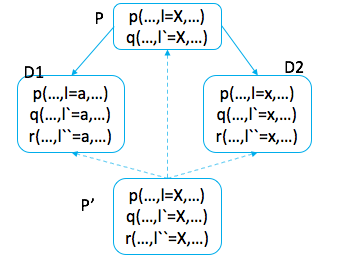
\includegraphics[width=250pt]{./pictures/0305.png}
\caption{Specific Pattern may exist}
\end{figure}
From the example we can see that, $D_1\preceq P$ is realized by $\theta_1= \{X=a\}$, and $D_2\preceq P$, by $X=x, Y=y$.\\
we can find a more specific $P' = {p(X,X),q(X)}$, makes that $D_1\preceq P$ but not $D_2\preceq P'$.\\
In a more simple situation, we may have two documents $D_1$ and $D_2$ , and a pattern $P$.
\begin{displaymath}
D_1 = \{p(l_1 = a, l_2 = a),q(l_1 = a)\}
\end{displaymath}
\begin{displaymath}
D_2 = \{p(l_1 = x, l_2 = y),q(l_1 = x)\}
\end{displaymath}
\begin{displaymath}
P = \{p(l_1 = X, l_2 = Y),q(l_1 = X)\}
\end{displaymath}
Thus, $a\in D_1$ and $x\in D_2$ plays the same role $ A_1 = {p(l_1),q(l_1)}$ represented by variable $X$.\\
As another shared role, $A_2 = {p(l_2)}$ , played by $a\in D_1$ and $y\in D_2$ and corresponding to $Y$.
Similarity class is a set of constants that play the same role $R \subseteq \mathcal{R}$ defined by the descriptive pattern. Durning the search process for the descriptive pattern, the exact similarity classes are also under investigation. We use the following sufficient condition for the similarity defined by the descriptive pattern.
\begin{enumerate}
\item for patterns $P_1\prec P_2$ realized by variable substitution $\theta$,
\begin{displaymath}
role_{P_2} (X) \subset role_{P_1} (X\theta)\ for\ X \in Var(P_2)
\end{displaymath}
That means role set represented by variable increases by specialization.
\item for a role set $\mathcal{R}$ ,we have
\begin{displaymath}
|[R]| = \{D\in \mathcal{D}|\psi_DR\ne \emptyset\}
\end{displaymath}
and,
\begin{displaymath}
|[R]| = \{D\in \mathcal{D}|\psi_DR\ne \emptyset\ and \ \max_{a\in const(D)}keyscore_D(a)\leq \kappa\}
\end{displaymath}
\item for a descriptive pattern $P$ and variable $X \in Var(P)$ , $R = role_P (X)$ is a maximal role set among role set $R'$, generated by a pattern. 
\end{enumerate}
Support $\mathcal{R}$ is a role set from descriptive pattern $P$ , if we can find a more specific $P'$ , it will lead inconsistency if the role set is not maximal. To make sure pattern $P$ is minimal among all satisfying ones, we have to maximize role set.\\
\begin{figure}[!h]
\centering
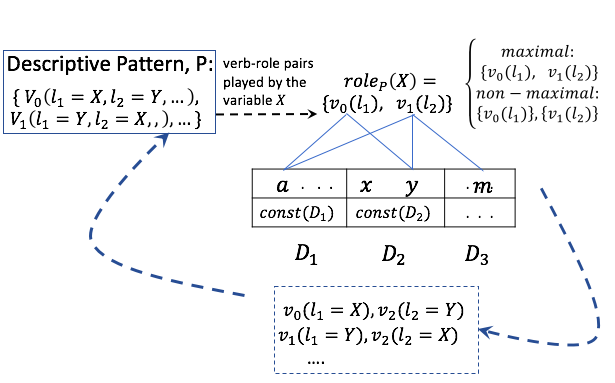
\includegraphics[width=300pt]{./pictures/0305-0.png}
\caption{Maximal closure is a complete set}
\end{figure}
We can use both Formal Concept Analysis or CLIQUE idea to extract maximal role set from our data. In my research, we use bipartite clique idea to solve the problem, because it is a more simple idea to understand the input and output, without learning more specific knowledge. We can understand the idea of bipartite clique to extract maximal closure of role set in the figure below,\\
\begin{figure}[!h]
\centering
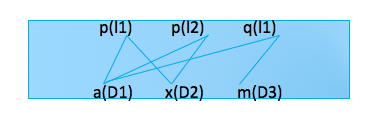
\includegraphics[width=250pt]{./pictures/0305-1.png}
\caption{there exists maximal bipartite clique with role set smaller than others}
\end{figure}
\begin{fact}
Actually, Maximal clique and Formal Concept have the same meaning. consider bipartite graph $(const(D),R,E)$ , where incident rel $E\subseteq const(D) \times R$ is defined by
\begin{displaymath}
C \iff FC<C \cap const(D),C\cap R>
\end{displaymath}
\end{fact}
\begin{proof}Sufficiency and Necessary,\\
Sufficiency: We cannot add new $D$ or $R$ elements to $C$. Hence, letting $A = C\cap R$,
\begin{displaymath}
\psi A = C\cap const(D)\ and\ A = \varphi\psi A
\end{displaymath}
Necessary: for $A = C \cap R$ and $\psi A = C \cap const(D)$ , as $A$ is a closure, we cannot add new role. as $\psi A$ is also an object closure, we cannot add new const.
\end{proof}
The processing of maximizing role set is as follow,\\
initial candidate set ${p(l)||[p(l)]| >\kappa}$,
\begin{displaymath}
Cand(R) = \{a\ role\ p(l)\notin R||D\in\mathcal{D}|\psi(R\cup\{p(l)\})\cap const(D)\ne \emptyset \}\ne N_\tau \}
\end{displaymath}
Of course, the candidate should meet the condition of KeyGraph,
\begin{displaymath}
maxKeyscore(\psi(R\cup\{p(l)\})\cap const(D))\geq\kappa
\end{displaymath}
\section{Re-construction of Descriptive Patterns}
\begin{figure}[!h]
\centering
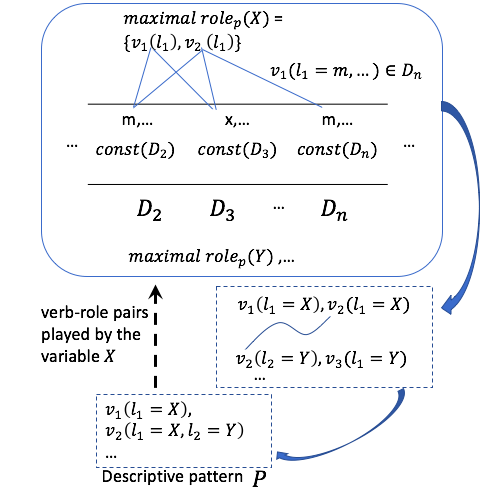
\includegraphics[width=250pt]{./pictures/0306.png}
\caption{primitive patterns and closures}
\end{figure}
If a pattern $P  = \{...,p(...,l = X,...),...\}$ can be a descriptive pattern, it should be with a maximal role set of variables $X,...(role_p (X),...)$ , and it should meet the condition of minisup. Using a Formal Concept Analysis Algorithm we can get the maximal closure $role_P (X)$ of the target descriptive pattern. The $role_P (X)$ meet the condition of minsup the descriptive pattern re-construct by it will also meet the condition of minsup. We can explain our idea in a figure.\\
We  have primitive pattern for closures,
\begin{displaymath}
pp(X) = v_1(l_1 = X), v_2(l_1 = X),...
\end{displaymath}
Although extracting all descriptive patterns will be a very difficult work depending on the document set we choose, by enlargement of role set and get maximal closures of $role_P (X)$ , the argument in $pp(X)$ is extended. That means more specific patterns can be extracted. Every possible specific pattern can be extracted from closures.\\
\begin{figure}[!h]
\centering
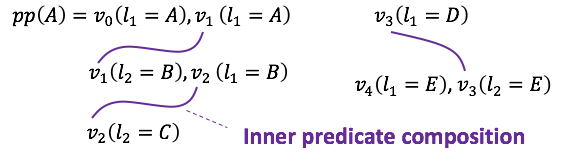
\includegraphics[width=300pt]{./pictures/0306-1.png}
\caption{Inner predicate composition}
\end{figure}
We have talked about the degree of difficulty to extract all descriptive patterns from maximal closure, but we can generate some representative descriptive pattern by some method. We have introduced KeyGraph Algorithm in the chapter before. And understand the association value between different nouns. Connecting same verbs in the primitive pattern set means to find a strong connection between the nouns, we always connect the highest association value pair one by one, until we cannot find other connections, we can understand this process in a figure.\\
Here is the detail process for this part, re-construct descriptive patterns $P$ with maximal closure set $C$.\\
We have a maximal closure set, We will have the primitive pattern for each closure.\\
\begin{displaymath}
pp(X) = v_1(l_1 = X), v_2 (l_1 = X)...
\end{displaymath}
\begin{displaymath}
pp(Y) = v_2(l_2 =Y),...
\end{displaymath}
Our purpose is to connect the verb-cases in primitive patterns to build the descriptive pattern. For each variable:
\begin{displaymath}
X, Y,... :X = {x_1, x_2,....}
\end{displaymath}
First we should find all the workable connections:
\begin{displaymath}
v1:\{\},v2:\{X,Y\},...
\end{displaymath}
We define the distance of the variables as the association value defined by KeyGraph Algorithm,
\begin{displaymath}
distance(X, Y) = \sum_{x_i \in X, y_i \in Y} association(x_i, y_i)
\end{displaymath}
Rank the value of distance, connect the strongest one. Then kick out the connected ones, repeat the process again. Finishing the whole processing, we will get one descriptive pattern if we always choose the strongest connection from our maximal closure set.\\
As the inner predicate composition is just a recover of the co-occurrence of nouns, we can use a breadth first algorithm to extract all possible descriptive patterns. The breadth first algorithm may take a large space and runtime, we propose beam search algorithm to help us pikc some main descriptive pattern from some sense.
As the association value recover the co-occurrence of nouns we have introduced, we also explained the Beam Search Algorithm in the former section. we can combine them together to get more than one Descriptive Patterns form a maximal closure set.\\
\begin{figure}[!h]
\centering
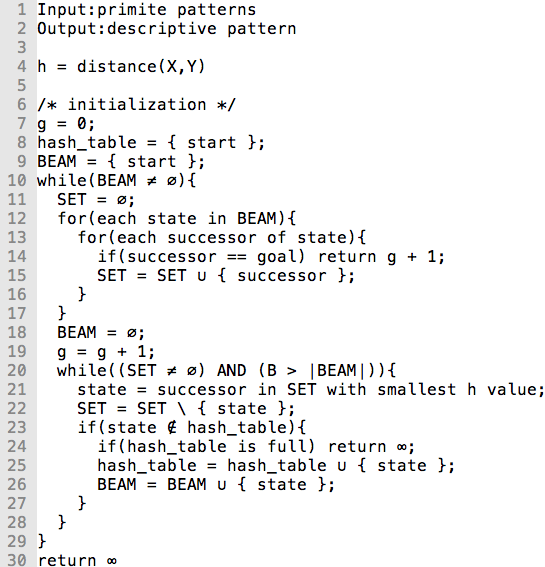
\includegraphics[width=250pt]{./pictures/0306-2.png}
\caption{Beam Search for re-construct descriptive patterns}
\end{figure}

\chapter{Experiment}
\section{Preprocessing}
We use four different kinds of data in our experiment:\\
Experiment 1: prove the feasibility of KeyGraph Algorithm.\\
Experiment 2: Using the whole set of document to experiment and assess the runtime of proposed algorithm.\\
Experiment 3: a set of two short Japanese stories, and set $\tau = 1$.\\
Experiment 4-1: a set of four similar precedent documents, and set $\tau = 1$.\\
Experiment 4-2: a set of four different precedent documents, and set $\tau = 1/2$ .\\
Experiment 4-3: a set of three precedent documents include similar and different ones, and set $\tau = 2/3$.\\
First, we need to transform the code of text to utf-8, we use Python language:\\
\begin{enumerate}[*]
\item import codecs
\item infile = codecs.open(`input',`r',`Shift JIS')
\item outfile = codecs.open(`output',`w',`utf-8')
\end{enumerate}
Then the files can be accessed by KNP system, we also need to piece the document to sentences to get a correct result from KNP system:\\
\begin{enumerate}[*]
\item sentences = document.split(`\begin{CJK}{UTF8}{ipxm}。\end{CJK}')
\end{enumerate}
Here, we use `\begin{CJK}{UTF8}{ipxm}。\end{CJK}' as a symbol of the end of a sentence. Because of precedents contains only declarative sentence, this simple way can solve the problem very fast and easily.
Then we can use KNP system to analysis our sentences with the command:\\
\begin{enumerate}[*]
\item `sentence' $|$ juman $|$ knp -simple
\end{enumerate}

For each document, we have a file to save KNP result.\\
Here are examples from the KNP result:\\
\begin{enumerate}[*]
\item \begin{CJK}{UTF8}{ipxm}
`目録 もくろく 目録 名詞 6 普通名詞 1 * 0 * 0 "代表表記:目録/もくろく カテゴリ:抽象物" '
\end{CJK}
\end{enumerate}
from lines of this kind, we can extract all nouns and use them to extract keyword using KeyGraph Algorithm.\\
\begin{enumerate}[*]
\item \begin{CJK}{UTF8}{ipxm}
`<格解析結果:操業/そうぎょう:動7:ガ/N/被告/0/0/1;...'
\end{CJK}
\end{enumerate}
from lines of this kind, we can extract the events.\\
With the keywords and all the events, we can start our experiment.\\
\section{KeyGraph Importacne}
We use KeyGraph Algorithm to improve the effectiveness and quality of our experiment, as we know if we use KeyGraph Algorithm to extract keywords, and disregards others, some information will be lost. It is very necessary to verify that after the processing of KeyGraph Algorithm, the result is still complete and powerful.\\
In this experiment to verify KeyGraph, we use some precedents downloaded from D1.com to see how KeyGraph will influence the connections between events. Whether the quality of events is influenced by disregarding some nouns.\\ \\
\textbf{Experiment}\\ \\
\begin{table}[!h]
\centering
\begin{tabular}{ccc}
\hline
Serial number&Precedent ID&Precedent Name\\
068&28110821&\begin{CJK}{UTF8}{ipxm}損害賠償請求事件-中国残留孤児国賠訴訟\end{CJK}\\
069&28111682&\begin{CJK}{UTF8}{ipxm}損害賠償請求事件-損害賠償等請求事件\end{CJK}\\
085&28162030&\begin{CJK}{UTF8}{ipxm}損害賠償請求事件-独立当事者参加事件\end{CJK}\\
\hline
\end{tabular}
\end{table}
\\ \\
Using all KNP results of each document, find all of the events, and check the proportion of events connected by high KeyScore nouns.\\ \\ 
\textbf{Result}\\ \\
\begin{figure}[!h]
\centering
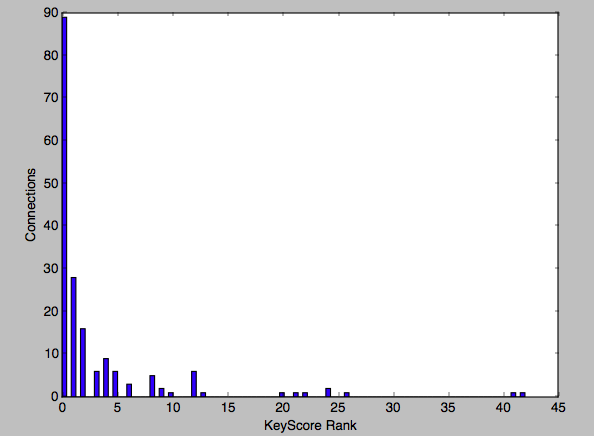
\includegraphics[width=300pt]{./pictures/0402-0.png}
\caption{Result of Experiment}
\end{figure}
The figure only shows top-45 rank KeyScore nouns because, after that, the connections between nouns are very less. And we can also find that main connections are between High KeyScore nouns, special top-25 ones. So in our experiment, we choose top-25 KeyScore nouns will be a very safe and efficient way.
\section{Experiment}
\textbf{Overview}
\\ \\
In this part we will talk about the whole experiment, lay aside the quality of the result, we mainly discuss the runtime from a grand view. We pick 30 precedents from our document set, and make an experiment to test the runtime of our algorithm in different situation. We have 3 sets of 10 precedents, 2 sets of 20 precedents, and 1 set of 30 precedents.\\
The result is as follow:\\
\begin{table}[!h]
\centering
\begin{tabular}{cccc}
\hline
Experiment&Event process&KeyGraph&MFC by CLIQUES\\
\hline
10-0&0.40&7.11&8.49\\
10-1&0.48&9.85&31.37\\
10-2&0.48&9.50&15.41\\
20-0&1.02&17.79&113.02\\
20-1&0.96&18.89&122.60\\
30-0&1.24&26.48&275.15\\
10-avg&0.45&8.82&18.42\\
20-avg&0.99&18.39&117.81\\
30-avg&1.24&26.48&275.15\\
\hline
\end{tabular}
\caption{data of runtime experiment}
\end{table}
We can find that the EVENT progress and KeyGraph algorithm is work in a linnner runtime, we the input increase, the runtime linear increases. But MFC by CLIQUE algorithm is different, when the amount of precedents increases, the runtime become very long and Increase rapidly.\\
 We can see it from a figure.\\ \\
\begin{figure}[!h]
\centering
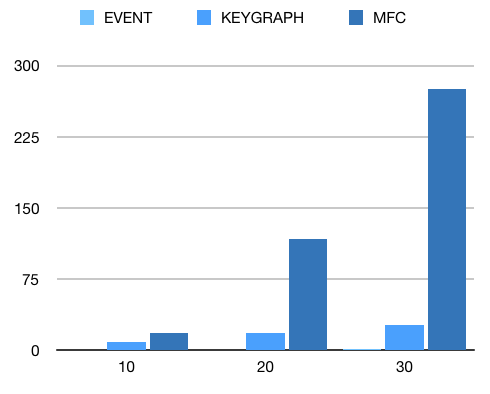
\includegraphics[width=250pt]{./pictures/0403-0.png}
\caption{statistic of runtime}
\end{figure}
After the evaluation, we mainly talk about the quality of the result in the following experiments, and what we can get from the algorithm.\\ \\
\textbf{Experiment of Short Japanese Stories}
\\ \\
We use the stories we have mentioned before, one is \begin{CJK}{UTF8}{ipxm}\textbf{あばれ鹿}\end{CJK} the other is \begin{CJK}{UTF8}{ipxm}\textbf{あやしい牛}\end{CJK}.\\
Because the stories is very short, the MFC founded is also very less, 4 result extracted:
\begin{enumerate}[*]
\item \begin{CJK}{UTF8}{ipxm}[荒らす/ヲ] [町001, 八百屋001, 田畑002]\end{CJK}
\item \begin{CJK}{UTF8}{ipxm}[持つ/ヲ] [光001, 火縄銃002]\end{CJK}
\item \begin{CJK}{UTF8}{ipxm}[困る/ガ] [若者001, 村人002]\end{CJK}
\item \begin{CJK}{UTF8}{ipxm}[現れる/ガ] [化け物001, 鹿002, 牛001, 老人001]\end{CJK}
\end{enumerate}
Although the result is not very well in this situation, we can still find some information from the result, some nouns play same role in different stories contain the information of descriptive similarity. The maximal closures will construct the descriptive pattern.
\begin{table}[!h]
\centering
\begin{tabular}{cc}
\hline
\begin{CJK}{UTF8}{ipxm}\textbf{あやしい牛}\end{CJK}&\begin{CJK}{UTF8}{ipxm}\textbf{あばれ鹿}\end{CJK}\\
\hline
\begin{CJK}{UTF8}{ipxm}町\end{CJK}&\begin{CJK}{UTF8}{ipxm}田畑\end{CJK}\\
\begin{CJK}{UTF8}{ipxm}若者\end{CJK}&\begin{CJK}{UTF8}{ipxm}村人\end{CJK}\\
\begin{CJK}{UTF8}{ipxm}光\end{CJK}&\begin{CJK}{UTF8}{ipxm}火縄銃\end{CJK}\\
\begin{CJK}{UTF8}{ipxm}牛\end{CJK}&\begin{CJK}{UTF8}{ipxm}鹿\end{CJK}\\
\hline
\end{tabular}
\caption{Similarity classes between stories}
\end{table}
\newpage
\textbf{Experiment 4-1}
\\ \\
In this experiment we use 4 similar precedents and set $\tau = 1$ to see whether there exist descriptive patterns supported by all the precedents.
\begin{table}[!h]
\centering
\begin{tabular}{cccc}
\hline
words(noun)&Event($s$)&KeyGraph($s$)&MFC($s$)\\
\hline
95423&0.22&16.77&28.89\\
\hline
\end{tabular}
\caption{4 similar Precedents}
\end{table}
51 maximal closures are extracted:
\begin{enumerate}
\item \begin{CJK}{UTF8}{ipxm}[有る/ニ, 言う/ト] [社会068, 項085, 過失092, 国保069]\end{CJK}
\item \begin{CJK}{UTF8}{ipxm}[受ける/ニ, 成る/ガ, 行う/ガ] [支部069, 株式085, 原告092, 原告068, 孤児068]\end{CJK}
\item \begin{CJK}{UTF8}{ipxm}[する/ニ, 受ける/カラ, 有る/ニ] [証券085, 国068, 原告092, 国保069]\end{CJK}
\item \begin{CJK}{UTF8}{ipxm}[する/ト, する/ヲ, つく/ニ, 成る/ガ, 認める/ガ] [義務068, 額085, 責任092, 被告069]\end{CJK}
\item \begin{CJK}{UTF8}{ipxm}[する/ト, つく/ニ, 成る/ガ, 有る/ガ, 認める/ガ] [義務068, 号085, 責任092, 被告069]\end{CJK}
\item \begin{CJK}{UTF8}{ipxm}[する/ガ, 主張/ガ, 求める/ガ, 生じる/ニ, 被る/ガ, 言う/ガ, 請求/ガ] [原告085, 原告092, 原告068, 国保069]\end{CJK}
\item \begin{CJK}{UTF8}{ipxm}[する/ガ, 有る/ニ, 認める/ニ, 請求/ガ] [原告085, 原告092, 被告069, 国068]\end{CJK}
\item \begin{CJK}{UTF8}{ipxm}[する/ガ, 主張/ガ, 有る/ニ, 求める/ガ, 生じる/ニ, 認める/ニ] [原告085, 原告092, 被告069, 被告068]\end{CJK}
\item \begin{CJK}{UTF8}{ipxm}[する/ガ, 検討/ガ, 求める/ガ, 生じる/ニ, 認める/ニ] [原告085, 原告092, 被告069, 孤児068]\end{CJK}
\item \begin{CJK}{UTF8}{ipxm}[する/ガ, する/ニ, 認める/ガ] [書069, 額085, 原告092, 過失092, 権利068, 号085, 士092]\end{CJK}
\item \begin{CJK}{UTF8}{ipxm}[する/ガ, つく/ニ, 成る/ガ] [法068, 株式085, 組合085, 額085, 責任092, 号085, 被告069]\end{CJK}
\item \begin{CJK}{UTF8}{ipxm}[する/ガ, 定める/ガ, 成る/ガ, 負う/ガ] [法068, 項085, 原告092, 国保069, 被告069]\end{CJK}
\item \begin{CJK}{UTF8}{ipxm}[する/ガ, 作成/ガ, 認識/ガ] [省068, 書085, 原告092, 国保069]\end{CJK}
\item \begin{CJK}{UTF8}{ipxm}[する/ガ, する/ニ, する/ヲ, 有る/ガ, 要求/ガ, 負う/ガ] [国068, 士092, 項085, 国保069]\end{CJK}
\item \begin{CJK}{UTF8}{ipxm}[する/ガ, する/ヲ, 有る/ガ, 要求/ガ, 認める/ニ, 負う/ガ] [国068, 士092, 項085, 被告069]\end{CJK}
\item \begin{CJK}{UTF8}{ipxm}[する/ガ, する/ニ, する/ヲ, 成る/ガ, 有る/ガ, 有る/ニ, 負う/ガ] [国068, 項085, 原告092, 国保069]\end{CJK}
\item \begin{CJK}{UTF8}{ipxm}[する/ガ, する/ヲ, 成る/ガ, 有る/ガ, 有る/ニ, 認める/ニ, 負う/ガ] [国068, 被告069, 項085, 原告092]\end{CJK}
\item \begin{CJK}{UTF8}{ipxm}[する/ガ, する/ニ, 受ける/カラ, 成る/ガ, 有る/ガ, 負う/ガ] [国068, 号085, 原告092, 国保069]\end{CJK}
\item \begin{CJK}{UTF8}{ipxm}[する/ガ, する/ニ, 含む/ガ, 有る/ニ] [国068, 書085, 原告092, 業務069]\end{CJK}
\item \begin{CJK}{UTF8}{ipxm}[する/ガ, する/ニ, 有る/ニ, 認識/ガ] [国068, 書085, 原告092, 国保069]\end{CJK}
\item \begin{CJK}{UTF8}{ipxm}[する/ガ, する/ヲ, 成る/ニ, 有る/ガ] [条092, 人068, 円085, 国保069]\end{CJK}
\item \begin{CJK}{UTF8}{ipxm}[する/ガ, する/ヲ, よる/ニ, 有る/ガ] [条092, 頁069, 項085, 者068]\end{CJK}
\item \begin{CJK}{UTF8}{ipxm}[する/ガ, 持つ/ヲ] [甲069, 株式085, 場092, 家族068, 責任092]\end{CJK}
\item \begin{CJK}{UTF8}{ipxm}[する/ガ, する/ト, 要する/ガ] [場092, 国保069, 項085, 人068]\end{CJK}
\item \begin{CJK}{UTF8}{ipxm}[する/ガ, する/ト, する/ニ, する/ヲ, 主張/ガ, 成る/ガ] [額085, 国保069, 原告092, 権利068]\end{CJK}
\item \begin{CJK}{UTF8}{ipxm}[する/ガ, する/ト, する/ヲ, 主張/ガ, 成る/ガ, 認める/ガ] [額085, 被告069, 原告092, 権利068]\end{CJK}
\item \begin{CJK}{UTF8}{ipxm}[する/ガ, する/ト, する/ヲ, 主張/ガ, 認める/ニ] [額085, 被告068, 原告092, 被告069]\end{CJK}
\item \begin{CJK}{UTF8}{ipxm}[する/ガ, する/ト, する/ヲ, つく/ニ, 認める/ガ] [額085, 条068, 責任092, 被告069]\end{CJK}
\item \begin{CJK}{UTF8}{ipxm}[する/ガ, する/ト, する/ヲ, 当たる/ガ, 成る/ガ] [線092, 被告069, 権利068, 円085, 者068]\end{CJK}
\item \begin{CJK}{UTF8}{ipxm}[する/ガ, する/ト, する/ヲ, 受ける/ガ, 成る/ガ] [株085, 原告092, 人068, 孤児068, 権利068, 者068, 国保069, 被告069]\end{CJK}
\item \begin{CJK}{UTF8}{ipxm}[する/ガ, する/ト, する/ニ, する/ヲ, 含む/ガ] [業務069, 円085, 原告092, 権利068, 者068]\end{CJK}
\item \begin{CJK}{UTF8}{ipxm}[する/ガ, する/ト, する/ヲ, 含む/ガ, 成る/ガ, 有る/ガ] [人068, 円085, 者068, 権利068, 原告092, 被告069]\end{CJK}
\item \begin{CJK}{UTF8}{ipxm}[する/ガ, する/ト, する/ニ, する/ヲ, 成る/ガ, 有る/ガ, 言う/ト] [過失092, 項085, 権利068, 国保069, 者068]\end{CJK}
\item \begin{CJK}{UTF8}{ipxm}[する/ガ, する/ト, する/ニ, する/ヲ, 成る/ガ, 有る/ガ, 生じる/ニ, 負う/ガ] [項085, 国保069, 孤児068, 原告092]\end{CJK}
\item \begin{CJK}{UTF8}{ipxm}[する/ガ, する/ト, する/ヲ, 成る/ガ, 有る/ガ, 生じる/ニ, 認める/ニ, 負う/ガ] [被告069, 項085, 原告092, 孤児068]\end{CJK}
\item \begin{CJK}{UTF8}{ipxm}[する/ガ, する/ト, する/ヲ, 定める/ガ, 有る/ガ, 有る/ニ, 生じる/ニ, 認める/ニ, 負う/ガ] [被告068, 項085, 原告092, 被告069]\end{CJK}
\item \begin{CJK}{UTF8}{ipxm}[する/ガ, する/ト, 成る/ガ, 有する/ガ, 行う/ガ] [株式085, 原告092, 被告069, 国保069, 孤児068, 者068]\end{CJK}
\item \begin{CJK}{UTF8}{ipxm}[する/ガ, する/ト, 主張/ガ, 行う/ガ] [株式085, 被告068, 原告092, 被告069, 国保069]\end{CJK}
\item \begin{CJK}{UTF8}{ipxm}[する/ガ, する/ト, 有する/ガ, 認める/ガ] [株式085, 条068, 被告069, 原告092]\end{CJK}
\item \begin{CJK}{UTF8}{ipxm}[する/ガ, する/ト, 成る/ト] [システム069, 額085, 者068, 権利068, 円085, 列車092, 人068, 孤児068]\end{CJK}
\item \begin{CJK}{UTF8}{ipxm}[する/ガ, する/ト, 有る/ガ, 認める/ガ, 負う/ガ] [号085, 士092, 原告092, 条068, 被告069]\end{CJK}
\item \begin{CJK}{UTF8}{ipxm}[する/ガ, する/ト, する/ニ, 成る/ガ, 有る/ガ, 言う/ガ] [号085, 者068, 原告092, 国保069]\end{CJK}
\item \begin{CJK}{UTF8}{ipxm}[する/ガ, する/ト, 成る/ガ, 有る/ガ, 認める/ガ] [号085, 責任092, 被告069, 原告092, 過失092, 権利068]\end{CJK}
\item \begin{CJK}{UTF8}{ipxm}[する/ガ, する/ト, 支払う/ガ, 有る/ガ, 負う/ガ] [号085, 被告068, 原告092, 国保069, 被告069]\end{CJK}
\item \begin{CJK}{UTF8}{ipxm}[する/ガ, する/ト, つく/ニ, 有る/ガ, 認める/ガ] [号085, 条068, 被告069, 責任092]\end{CJK}
\item \begin{CJK}{UTF8}{ipxm}[する/ガ, 主張/ガ, 成る/ガ, 有する/ガ, 行う/ガ] [原告068, 株式085, 原告092, 国保069, 被告069]\end{CJK}
\item \begin{CJK}{UTF8}{ipxm}[する/ガ, する/ヲ, 占める/ガ, 成る/ガ, 有る/ガ] [原告068, 被告069, 過失092, 円085]\end{CJK}
\item \begin{CJK}{UTF8}{ipxm}[する/ガ, する/ニ, 含む/ガ, 行う/ニ] [書085, 業務069, 原告092, 者068]\end{CJK}
\item \begin{CJK}{UTF8}{ipxm}[する/ガ, 含む/ガ, 有る/ニ, 行う/ニ, 認める/ニ] [書085, 被告068, 原告092, 被告069]\end{CJK}
\item \begin{CJK}{UTF8}{ipxm}[する/ガ, 提出/ガ, 行う/ニ, 認める/ニ] [書085, 士092, 被告069, 者068]\end{CJK}
\item \begin{CJK}{UTF8}{ipxm}[支払う/ガ, 求める/ニ, 負う/ガ] [被告085, 国保069, 被告068, 被告092, 被告069]\end{CJK}
\end{enumerate}
We can pick some closures to bulid part of our descriptive pattern manual, because the document is very similar, the pattern may very long, we list part of them.
\begin{figure}[!h]
\centering
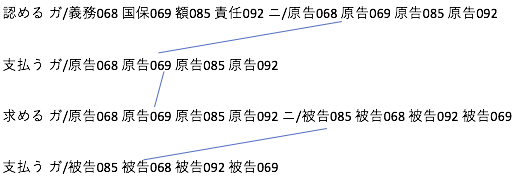
\includegraphics[width=250pt]{./pictures/0403-1.png}
\caption{Part of Descriptive patterns}
\end{figure}
\newpage
\textbf{Experiment 4-2}
\\ \\
In this experiment we use 4 precedents which seem very different from each other and set $\tau = 1/2$ to see whether our algorithm can extract descriptive patterns among multiple precedents.
\begin{table}[!h]
\centering
\begin{tabular}{cccc}
\hline
words(noun)&Event($s$)&KeyGraph($s$)&MFC($s$)\\
\hline
6974&0.03&0.40&0.09\\
\hline
\end{tabular}
\caption{4 very differnet Precedents}
\end{table}
Closures are extracted:
\begin{enumerate}
\item \begin{CJK}{UTF8}{ipxm}[受ける/ニ, 変更/ニ] [事件007, 人000]\end{CJK}
\item \begin{CJK}{UTF8}{ipxm}[喪失/ニ, 死亡/ニ] [事故077, 行為000]\end{CJK}
\item \begin{CJK}{UTF8}{ipxm}[主張/ガ, 居住/ガ, 請求/ニ] [被告007, 被告005]\end{CJK}
\item \begin{CJK}{UTF8}{ipxm}[する/ト, する/ニ] [権000, 原告007]\end{CJK}
\item \begin{CJK}{UTF8}{ipxm}[する/ト, 主張/ガ, 受ける/ガ, 受ける/ニ, 求める/ガ, 求める/ニ, 知る/ガ] [被告005, 原告007]\end{CJK}
\item \begin{CJK}{UTF8}{ipxm}[する/ト, 言う/ガ] [逸失利益000, 原告007]\end{CJK}
\item \begin{CJK}{UTF8}{ipxm}[する/ト, 考える/ガ] [逸失利益000, 口007]\end{CJK}
\item \begin{CJK}{UTF8}{ipxm}[する/ト, 成る/ガ, 生じる/ニ] [利益000, 原告007]\end{CJK}
\item \begin{CJK}{UTF8}{ipxm}[受ける/ニ, 請求/ニ] [行為007, 被告005]\end{CJK}
\item \begin{CJK}{UTF8}{ipxm}[求める/ガ, 求める/ニ, 請求/ニ] [人077, 被告005]\end{CJK}
\item \begin{CJK}{UTF8}{ipxm}[求める/ニ, 負う/ニ] [人077, 者000]\end{CJK}
\item \begin{CJK}{UTF8}{ipxm}[控訴/ガ, 求める/ガ, 求める/ニ] [人077, 原告007]\end{CJK}
\item \begin{CJK}{UTF8}{ipxm}[受ける/ガ, 受ける/ニ, 命ずる/ニ, 支払う/ガ, 求める/ガ] [人000, 原告007]\end{CJK}
\item \begin{CJK}{UTF8}{ipxm}[取得/ガ, 受ける/ガ, 受ける/ニ, 求める/ガ] [人000, 被告005]\end{CJK}
\item \begin{CJK}{UTF8}{ipxm}[有る/ガ, 生じる/ニ] [者000, 過失077]\end{CJK}
\item \begin{CJK}{UTF8}{ipxm}[受ける/ガ, 求める/ニ, 生じる/ニ, 被る/ガ, 負う/ガ] [者000, 原告007]\end{CJK}
\item \begin{CJK}{UTF8}{ipxm}[取得/ガ, 受ける/ガ, 求める/ニ] [者000, 被告005]\end{CJK}
\item \begin{CJK}{UTF8}{ipxm}[成る/ガ, 言う/ガ] [額000, 原告007]\end{CJK}
\item \begin{CJK}{UTF8}{ipxm}[する/ガ, する/ヲ, 言う/ガ] [額000, 事件005]\end{CJK}
\item \begin{CJK}{UTF8}{ipxm}[受ける/ニ, 言う/ガ] [事件005, 原告007]\end{CJK}
\end{enumerate}
Although the document are very different, we can still extract similarity classes between two of them, they can also build descriptive patterns.
\begin{figure}[!h]
\centering
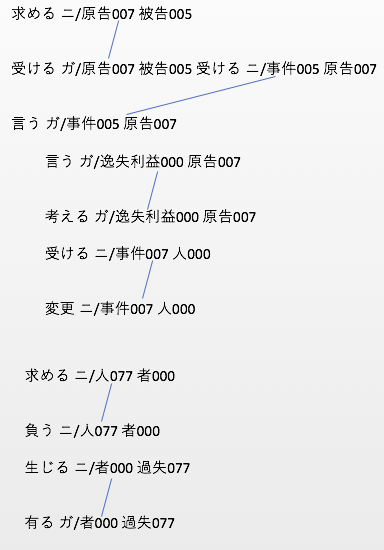
\includegraphics[width=250pt]{./pictures/0403-2.png}
\caption{Part of Descriptive patterns between different documents}
\end{figure}
\newpage
\textbf{Experiment 4-3}
\\ \\
In this experiment we use 3 precedents, two of them are similar ones and set $\tau = 2/3$. The propose is to see whether our algorithm can find similar ones between a document set.
\begin{table}[!h]
\centering
\begin{tabular}{cccc}
\hline
words(noun)&Event($s$)&KeyGraph($s$)&MFC($s$)\\
\hline
76083&0.15&10.31&8.27\\
\hline
\end{tabular}
\caption{3 Precedents include 2 similar ones}
\end{table}
Closures are extracted:
\begin{enumerate}
\item \begin{CJK}{UTF8}{ipxm}[する/デ, 取る/ニ, 有る/ニ] [駅092, 社会068]\end{CJK}
\item \begin{CJK}{UTF8}{ipxm}[する/ヲ, 取る/ニ, 書く/ニ, 有る/ガ, 設置/ニ, 連絡/ニ] [駅092, 省068]\end{CJK}
\item \begin{CJK}{UTF8}{ipxm}[する/ニ, する/ヲ, 取る/ニ, 成る/ガ, 有る/ガ, 発生/ガ, 至る/ニ, 行う/ニ] [駅092, 孤児068]\end{CJK}
\item \begin{CJK}{UTF8}{ipxm}[する/ニ, する/ヲ, 成る/ガ, 有る/ガ, 有る/ニ, 行う/デ] [駅092, 国068]\end{CJK}
\item \begin{CJK}{UTF8}{ipxm}[する/ヲ, 有る/ガ, 有る/ニ, 発生/ガ, 行う/ニ] [駅092, 被告068]\end{CJK}
\item \begin{CJK}{UTF8}{ipxm}[する/ニ, する/ヲ, 居る/ニ, 行う/ニ, 設置/ニ] [駅092, センター068]\end{CJK}
\item \begin{CJK}{UTF8}{ipxm}[する/ニ, する/ヲ, 成る/ガ, 置く/ニ, 行う/ニ] [駅092, 問題068]\end{CJK}
\item \begin{CJK}{UTF8}{ipxm}[する/デ, 受ける/ニ, 得る/ニ, 有る/ニ, 確立/ニ] [社会068, 原告092]\end{CJK}
\item \begin{CJK}{UTF8}{ipxm}[する/デ, 出来る/ニ, 取る/ニ, 持つ/ヲ] [社会068, 場092]\end{CJK}
\item \begin{CJK}{UTF8}{ipxm}[有る/ニ, 言う/ト] [社会068, 過失092]\end{CJK}
\item \begin{CJK}{UTF8}{ipxm}[持つ/ヲ, 言う/ト] [社会068, 責任092]\end{CJK}
\item \begin{CJK}{UTF8}{ipxm}[受ける/ニ, 発する/ガ] [騒音025, 原告092]\end{CJK}
\item \begin{CJK}{UTF8}{ipxm}[有る/ガ, 有る/ニ, 生じる/ニ, 発生/ガ, 発生/ニ, 行う/ニ, 認める/ニ] [事故092, 被告068]\end{CJK}
\item \begin{CJK}{UTF8}{ipxm}[する/ニ, 判断/ニ, 有る/ガ, 死亡/デ, 死亡/ニ, 生じる/ニ, 発生/ガ, 至る/ニ, 行う/ニ, 認める/ニ] [事故092, 者068]\end{CJK}
\item \begin{CJK}{UTF8}{ipxm}[する/ニ, 判断/ニ, 取る/ニ, 周知/ニ, 有る/ガ, 生じる/ニ, 発生/ガ, 発生/ヲ, 至る/ニ, 行う/ニ, 認める/ニ] [事故092, 孤児068]\end{CJK}
\item \begin{CJK}{UTF8}{ipxm}[する/ニ, 存在/ニ, 有る/ガ, 生じる/ニ, 発生/ガ, 発生/ニ] [事故092, 原告068]\end{CJK}
\item \begin{CJK}{UTF8}{ipxm}[知る/ヲ, 行う/ニ] [事故092, 身元068]\end{CJK}
\item \begin{CJK}{UTF8}{ipxm}[行う/ガ, 述べる/ガ] [谷092, 孤児068]\end{CJK}
\item \begin{CJK}{UTF8}{ipxm}[する/ニ, する/ヲ, 受ける/ニ, 行う/ガ, 行う/ニ, 設置/ガ, 運営/ガ] [センター068, 原告092]\end{CJK}
\item \begin{CJK}{UTF8}{ipxm}[行う/ガ, 行う/ニ, 設置/ガ, 設置/ニ] [センター068, 県092]\end{CJK}
\item \begin{CJK}{UTF8}{ipxm}[する/ニ, 出来る/ニ, 居る/ニ, 行う/ニ, 設置/ヲ] [センター068, 場092]\end{CJK}
\item \begin{CJK}{UTF8}{ipxm}[する/ヲ, 判断/ガ, 成る/ト, 持つ/カラ, 行う/ニ] [円092, 者068]\end{CJK}
\item \begin{CJK}{UTF8}{ipxm}[する/ヲ, 行う/ニ, 鳴る/ト] [円092, 家族068]\end{CJK}
\item \begin{CJK}{UTF8}{ipxm}[する/ヲ, 主張/ガ, 成る/ト] [円092, 権利068]\end{CJK}
\item \begin{CJK}{UTF8}{ipxm}[する/ヲ, 認める/ト] [円092, 義務068]\end{CJK}
\item \begin{CJK}{UTF8}{ipxm}[する/ト, する/ニ, する/ヲ, 取る/ガ, 成る/ガ, 指摘/ガ, 行う/ニ, 認識/ガ, 負う/ガ] [問題068, 原告092]\end{CJK}
\item \begin{CJK}{UTF8}{ipxm}[する/ト, する/ニ, する/ヲ, 取る/ガ, 提出/ガ, 行う/ニ, 認識/ガ, 負う/ガ] [問題068, 士092]\end{CJK}
\item \begin{CJK}{UTF8}{ipxm}[する/ト, する/ニ, する/ヲ, 成る/ガ, 起こす/ニ] [問題068, 過失092]\end{CJK}
\item \begin{CJK}{UTF8}{ipxm}[する/ト, 成る/ガ, 提出/ガ, 置く/ニ, 行う/ニ] [問題068, 県092]\end{CJK}
\item \begin{CJK}{UTF8}{ipxm}[する/ト, する/ニ, 置く/ニ, 行う/ニ] [問題068, 場092]\end{CJK}
\item \begin{CJK}{UTF8}{ipxm}[受ける/カラ, 受ける/ガ, 求める/カラ] [住民025, 原告092]\end{CJK}
\item \begin{CJK}{UTF8}{ipxm}[する/ト, する/ヲ, つく/ニ, 合う/ガ, 履行/ヲ, 怠る/ヲ, 有る/ガ, 規定/ガ, 認める/ヲ, 課す/ヲ, 課する/ヲ, 負う/ヲ, 違反/ニ] [義務068, 義務092]\end{CJK}
\item \begin{CJK}{UTF8}{ipxm}[する/ト, する/ヲ, 主張/ヲ, 存在/ガ, 成る/ガ, 有る/ガ, 認める/ガ, 認める/ヲ] [義務068, 過失092]\end{CJK}
\item \begin{CJK}{UTF8}{ipxm}[する/ト, する/ヲ, つく/ニ, 成る/ガ, 有る/ガ, 認める/ガ, 認める/ヲ, 負う/ヲ] [義務068, 責任092]\end{CJK}
\item \begin{CJK}{UTF8}{ipxm}[する/ト, する/ヲ, 合う/ガ, 成る/ガ, 有る/ガ, 認める/ガ, 課する/ガ] [義務068, 原告092]\end{CJK}
\item \begin{CJK}{UTF8}{ipxm}[する/ヲ, 定める/ヲ, 有る/ガ, 規定/ガ, 規定/ニ, 規定/ヲ, 違反/ニ] [義務068, 条092]\end{CJK}
\item \begin{CJK}{UTF8}{ipxm}[発生/ガ, 認める/ガ] [義務068, 本件092]\end{CJK}
\item \begin{CJK}{UTF8}{ipxm}[有る/ガ, 考慮/ヲ] [義務068, 要素025]\end{CJK}
\item \begin{CJK}{UTF8}{ipxm}[締結/ガ, 行う/デ, 認める/ニ] [本件092, 国068]\end{CJK}
\item \begin{CJK}{UTF8}{ipxm}[発生/ガ, 認める/ニ, 違反/ガ] [本件092, 被告068]\end{CJK}
\item \begin{CJK}{UTF8}{ipxm}[発生/ガ, 至る/ガ, 認める/ニ] [本件092, 孤児068]\end{CJK}
\item \begin{CJK}{UTF8}{ipxm}[共通/ガ, 有る/ガ] [要素025, 権利068, 原告068]\end{CJK}
\item \begin{CJK}{UTF8}{ipxm}[する/ガ, 定める/ガ, 定める/ニ, 規定/ガ, 規定/ニ, 規律/ガ, 適用/ガ] [法068, 条092]\end{CJK}
\item \begin{CJK}{UTF8}{ipxm}[する/ガ, 受ける/ガ, 定める/ガ, 成る/ガ, 負う/ガ, 負う/ニ, 足る/ガ] [法068, 原告092]\end{CJK}
\item \begin{CJK}{UTF8}{ipxm}[する/ガ, 主張/ヲ, 成る/ガ, 負う/ニ] [法068, 過失092]\end{CJK}
\item \begin{CJK}{UTF8}{ipxm}[する/ガ, つく/ニ, 成る/ガ, 成立/ガ, 負う/ト, 負う/ニ] [法068, 責任092]\end{CJK}
\item \begin{CJK}{UTF8}{ipxm}[する/ガ, 発生/カラ] [法068, 場092]\end{CJK}
\item \begin{CJK}{UTF8}{ipxm}[する/ガ, 主張/ヲ, 受ける/ガ, 負う/ガ] [法068, 士092]\end{CJK}
\item \begin{CJK}{UTF8}{ipxm}[する/ガ, 有る/ガ, 至る/ニ] [被害025, 者068, 孤児068]\end{CJK}
\item \begin{CJK}{UTF8}{ipxm}[する/ガ, 受ける/ヲ, 有る/ガ] [被害025, 省068]\end{CJK}
\item \begin{CJK}{UTF8}{ipxm}[する/ガ, する/ト, 出来る/ガ, 存在/ガ, 射る/ガ, 居る/ガ, 成る/ガ, 成る/ト, 行う/ニ, 言う/ト] [列車092, 人068]\end{CJK}
\item \begin{CJK}{UTF8}{ipxm}[する/ガ, する/ト, 与える/ニ, 出す/ヲ, 出来る/ガ, 存在/ガ, 居る/ガ, 成る/ガ, 成る/ト, 発生/ガ, 編成/ヲ, 行う/ニ, 言う/ト] [列車092, 者068]\end{CJK}
\item \begin{CJK}{UTF8}{ipxm}[する/ガ, する/ト, 出す/ヲ, 出来る/ガ, 存在/ガ, 居る/ガ, 差し掛かる/ガ, 待つ/ガ, 成る/ガ, 成る/ト, 発生/ガ, 行う/ニ, 遅れる/ガ] [列車092, 孤児068]\end{CJK}
\item \begin{CJK}{UTF8}{ipxm}[する/ガ, 出来る/ガ, 居る/ガ, 待つ/ガ, 待つ/ヲ, 成る/ガ, 発生/ガ, 遅れる/ガ] [列車092, 原告068]\end{CJK}
\item \begin{CJK}{UTF8}{ipxm}[する/ガ, する/ヲ, 定める/ガ, 有る/ガ, 構成/ガ, 確認/ガ, 行う/ト] [省068, 条092]\end{CJK}
\item \begin{CJK}{UTF8}{ipxm}[する/ガ, する/ヲ, 作成/ガ, 受ける/ガ, 報告/ニ, 定める/ガ, 実施/ガ, 持つ/ガ, 有る/ガ, 行う/ト, 認める/ガ, 認識/ガ, 連絡/ニ] [省068, 原告092]\end{CJK}
\item \begin{CJK}{UTF8}{ipxm}[する/ガ, する/ヲ, 受ける/ガ, 有る/ガ, 確認/ガ, 認める/ガ, 認識/ガ] [省068, 士092]\end{CJK}
\item \begin{CJK}{UTF8}{ipxm}[する/ガ, する/ヲ, 有る/ガ, 認める/ガ, 軽視/ガ] [省068, 責任092]\end{CJK}
\item \begin{CJK}{UTF8}{ipxm}[する/ガ, する/ト, する/ヲ, つく/ニ, 有る/ガ, 規定/ガ, 違反/ニ] [義務092, 条068]\end{CJK}
\item \begin{CJK}{UTF8}{ipxm}[する/ガ, する/ト, する/ヲ, 会う/ガ, 有る/ガ, 規定/ガ, 認める/ヲ] [義務092, 者068]\end{CJK}
\item \begin{CJK}{UTF8}{ipxm}[する/ガ, する/ト, する/ヲ, 有る/ガ, 発生/ヲ, 負う/ヲ] [義務092, 孤児068]\end{CJK}
\item \begin{CJK}{UTF8}{ipxm}[する/ガ, する/ト, する/ヲ, つく/ニ, 有る/ガ, 言う/ト, 認める/ガ, 負う/ト, 負う/ニ] [条068, 責任092]\end{CJK}
\item \begin{CJK}{UTF8}{ipxm}[する/ガ, する/ト, する/ヲ, 含む/ガ, 定める/ガ, 有する/ガ, 有する/ニ, 有る/ガ, 行う/ニ, 要請/ガ, 認める/ガ, 負う/ガ, 負う/ニ, 負担/ニ] [条068, 原告092]\end{CJK}
\item \begin{CJK}{UTF8}{ipxm}[する/ガ, する/ト, する/ヲ, 実現/ガ, 有る/ガ, 生じる/カラ, 行う/ニ, 認める/ガ, 負う/ガ] [条068, 士092]\end{CJK}
\item \begin{CJK}{UTF8}{ipxm}[する/ガ, する/ト, する/ヲ, 成る/ガ, 有る/ガ, 止まる/ガ, 言う/ト, 認める/ヲ, 負う/ニ] [責任092, 者068]\end{CJK}
\item \begin{CJK}{UTF8}{ipxm}[する/ガ, する/ト, する/ニ, する/ヲ, 存在/ガ, 成る/ガ, 有る/ガ, 言う/ト, 認める/ニ, 認める/ヲ, 負う/ニ] [過失092, 者068]\end{CJK}
\item \begin{CJK}{UTF8}{ipxm}[する/ガ, する/ト, する/ニ, する/ヲ, 合わせる/ヲ, 成る/ガ, 有る/ガ, 言う/ト, 認める/ガ, 認める/ヲ] [過失092, 権利068]\end{CJK}
\item \begin{CJK}{UTF8}{ipxm}[する/ガ, する/ト, する/ニ, する/ヲ, 主張/ガ, 反する/ガ, 受ける/ガ, 含む/ガ, 成る/ガ, 有る/ガ, 認める/ガ] [原告092, 権利068]\end{CJK}
\item \begin{CJK}{UTF8}{ipxm}[する/ガ, する/ト, する/ヲ, 区分/ガ, 取る/ガ, 受ける/ガ, 含む/ガ, 居る/ガ, 成る/ガ, 有る/ガ, 果たす/ガ, 行う/ガ, 行う/ニ, 言う/ガ, 鳴る/デ] [原告092, 人068]\end{CJK}
\item \begin{CJK}{UTF8}{ipxm}[する/ガ, する/ト, する/ニ, する/ヲ, 保有/ガ, 出す/カラ, 出す/ガ, 取得/ガ, 受ける/ガ, 含む/ガ, 居る/ガ, 得る/ニ, 成る/ガ, 持つ/ガ, 提出/カラ, 有する/ガ, 有する/ニ, 有る/カラ, 有る/ガ, 求める/カラ, 求める/ガ, 生じる/ニ, 知る/ガ, 立てる/ガ, 行う/ガ, 行う/ニ, 見る/ガ, 言う/ガ, 該当/ガ, 認める/ニ, 負う/ニ] [原告092, 者068]\end{CJK}
\item \begin{CJK}{UTF8}{ipxm}[する/ガ, する/ト, する/ニ, する/ヲ, 保有/ガ, 取る/ガ, 受ける/ガ, 受ける/ニ, 居る/ガ, 得る/ニ, 成る/ガ, 拒否/ガ, 持つ/ガ, 有する/ガ, 有する/ニ, 有る/ガ, 検討/ガ, 求める/ガ, 生じる/ニ, 知る/ガ, 確立/ニ, 罹る/ガ, 至る/ガ, 行う/カラ, 行う/ガ, 行う/ニ, 行使/ガ, 認める/ニ, 負う/ガ, 負担/ガ] [原告092, 孤児068]\end{CJK}
\item \begin{CJK}{UTF8}{ipxm}[する/ガ, する/ト, する/ニ, する/ヲ, 存在/ガ, 成る/ガ, 有る/ガ, 検討/ガ, 認める/ニ] [孤児068, 過失092]\end{CJK}
\item \begin{CJK}{UTF8}{ipxm}[する/ガ, する/ト, する/ヲ, 成る/ガ, 有る/ガ, 負う/ヲ] [孤児068, 責任092]\end{CJK}
\item \begin{CJK}{UTF8}{ipxm}[する/ガ, する/ト, する/ヲ, 与える/ニ, 取る/ガ, 採る/ガ, 有る/ガ, 求める/ニ, 行う/ガ, 行う/ニ, 認める/ニ, 認識/ガ, 課する/ニ, 負う/ガ] [士092, 被告068]\end{CJK}
\item \begin{CJK}{UTF8}{ipxm}[する/ガ, する/ト, する/ヲ, 乗る/ガ, 入る/ガ, 取る/ガ, 受ける/ガ, 居る/ガ, 戻る/ガ, 有る/ガ, 聞く/カラ, 聞く/ガ, 行う/ガ, 行う/ニ, 言う/ガ] [士092, 人068]\end{CJK}
\item \begin{CJK}{UTF8}{ipxm}[する/ガ, する/ト, する/ニ, する/ヲ, 取る/ガ, 受ける/ガ, 居る/ガ, 強いる/ニ, 有る/ガ, 確認/ガ, 聞く/カラ, 行う/ガ, 行う/ニ, 認める/ニ, 負う/ガ] [士092, 孤児068]\end{CJK}
\item \begin{CJK}{UTF8}{ipxm}[する/ガ, する/ト, する/ニ, する/ヲ, 与える/ニ, 出す/カラ, 受ける/ガ, 居る/ガ, 戻る/ガ, 提出/ガ, 有る/ガ, 確認/ガ, 行う/ガ, 行う/ニ, 見る/ガ, 言う/ガ, 認める/ニ] [士092, 者068]\end{CJK}
\item \begin{CJK}{UTF8}{ipxm}[する/ガ, する/ト, する/ニ, する/ヲ, 受ける/ガ, 戻る/ガ, 有る/ガ, 認める/ガ] [士092, 権利068]\end{CJK}
\item \begin{CJK}{UTF8}{ipxm}[する/ガ, する/ト, する/ヲ, 主張/ガ, 予見/ガ, 作る/ガ, 取る/ガ, 合う/ガ, 含む/ガ, 定める/ガ, 実施/ガ, 持つ/ガ, 指摘/ガ, 挙げる/ガ, 採る/ガ, 支払う/ガ, 放棄/ガ, 有る/ガ, 有る/ニ, 果たす/ガ, 求める/ガ, 派遣/ガ, 生じる/ニ, 申し入れる/ガ, 続ける/ガ, 行う/ガ, 行う/ニ, 設置/ガ, 認める/ニ, 認識/ガ, 負う/ガ, 負う/ニ, 違反/ガ] [被告068, 原告092]\end{CJK}
\item \begin{CJK}{UTF8}{ipxm}[する/ガ, する/ニ, する/ヲ, よる/ニ, 明らかだ/ガ, 明確だ/ニ, 有る/ガ, 生じる/ニ, 確認/ガ, 確認/ニ, 行う/ニ, 規定/ガ, 規定/ニ] [条092, 者068]\end{CJK}
\item \begin{CJK}{UTF8}{ipxm}[する/ガ, する/ニ, する/ヲ, 明らかだ/ガ, 有る/ガ, 有る/ニ, 規定/ニ] [条092, 国068]\end{CJK}
\item \begin{CJK}{UTF8}{ipxm}[する/ガ, する/ニ, する/ヲ, 有る/ガ, 適用/ガ] [条092, 権利068]\end{CJK}
\item \begin{CJK}{UTF8}{ipxm}[する/ガ, する/ヲ, 定める/ガ, 定める/ニ, 有る/ガ, 行う/ニ, 規定/ガ, 規定/ニ, 規定/ヲ, 言う/ニ, 違反/ニ] [条092, 条068]\end{CJK}
\item \begin{CJK}{UTF8}{ipxm}[する/ガ, する/ヲ, 成る/ニ, 有る/ガ, 行う/ニ, 規定/ガ] [条092, 人068]\end{CJK}
\item \begin{CJK}{UTF8}{ipxm}[する/ガ, する/ニ, する/ヲ, 伝える/ニ, 反する/ガ, 受ける/カラ, 受ける/ガ, 含む/ガ, 実施/ガ, 成る/ガ, 有する/ガ, 有る/ガ, 有る/ニ, 果たす/ガ, 申し立てる/ガ, 究明/ガ, 行う/ガ, 認める/ニ, 認識/ガ, 課す/ニ, 請求/ガ, 負う/ガ, 負担/ガ, 負担/ニ, 進める/ニ, 開設/ニ] [国068, 原告092]\end{CJK}
\item \begin{CJK}{UTF8}{ipxm}[する/ガ, する/ニ, する/ヲ, 受ける/ガ, 有る/ガ, 行う/ガ, 要求/ガ, 認める/ニ, 認識/ガ, 課す/ニ, 負う/ガ] [国068, 士092]\end{CJK}
\item \begin{CJK}{UTF8}{ipxm}[する/ガ, する/ニ, する/ヲ, 主張/ヲ, 占める/ガ, 合わせる/ヲ, 成る/ガ, 有る/ガ] [原告068, 過失092]\end{CJK}
\item \begin{CJK}{UTF8}{ipxm}[する/ガ, する/ニ, する/ヲ, 主張/ガ, 出す/ガ, 取る/ガ, 取得/ガ, 受ける/ガ, 受ける/ニ, 含む/ガ, 居る/ガ, 成る/ガ, 持つ/ガ, 指摘/ガ, 挙げる/ガ, 有する/ガ, 有る/ガ, 果たす/ガ, 求める/ガ, 生じる/ニ, 確立/ガ, 続ける/ガ, 行う/ガ, 行使/ガ, 被る/ガ, 見る/ガ, 言う/ガ, 請求/ガ, 足る/ガ] [原告068, 原告092]\end{CJK}
\item \begin{CJK}{UTF8}{ipxm}[する/ガ, する/ニ, する/ヲ, 主張/ヲ, 取る/ガ, 受ける/ガ, 対する/ニ, 居る/ガ, 有る/ガ, 行う/ガ, 要求/ガ, 見る/ガ, 言う/ガ] [原告068, 士092]\end{CJK}
\item \begin{CJK}{UTF8}{ipxm}[する/ガ, する/ト, する/ヲ, 与える/ニ, 出す/カラ, 当たる/ガ, 有する/ガ, 行う/ニ] [被告092, 者068]\end{CJK}
\item \begin{CJK}{UTF8}{ipxm}[する/ガ, する/ト, する/ヲ, 与える/ニ, 主張/ガ, 委託/ガ, 履行/ガ, 支払う/ガ, 放棄/ガ, 求める/ニ, 行う/ニ, 負う/ガ] [被告092, 被告068]\end{CJK}
\item \begin{CJK}{UTF8}{ipxm}[する/ガ, する/ト, する/ヲ, 主張/ガ, 当たる/ガ] [被告092, 権利068]\end{CJK}
\item \begin{CJK}{UTF8}{ipxm}[する/ガ, する/ヲ, 主張/ガ, 付く/ガ, 存在/ニ, 有する/ガ, 知る/ニ, 行使/ガ] [被告092, 原告068]\end{CJK}
\item \begin{CJK}{UTF8}{ipxm}[する/ガ, する/ヲ, 否定/ガ, 有る/ニ, 認める/ガ] [原判決025, 原告092, 過失092]\end{CJK}
\item \begin{CJK}{UTF8}{ipxm}[する/ガ, する/デ, する/ト, する/ニ, する/ヲ, 出す/カラ, 受ける/ガ, 同意/ガ, 居る/ガ, 有る/カラ, 知る/ガ, 行う/ニ, 行う/ヲ] [家族068, 原告092]\end{CJK}
\item \begin{CJK}{UTF8}{ipxm}[する/ガ, する/ト, する/ニ, する/ヲ, 出す/カラ, 受ける/ガ, 居る/ガ, 求める/ニ, 行う/ニ] [家族068, 士092]\end{CJK}
\item \begin{CJK}{UTF8}{ipxm}[する/ガ, する/ト, する/ヲ, 持つ/ヲ] [家族068, 責任092]\end{CJK}
\item \begin{CJK}{UTF8}{ipxm}[する/ガ, する/ヲ, 報告/ニ, 設置/ニ] [線092, 省068]\end{CJK}
\item \begin{CJK}{UTF8}{ipxm}[する/ガ, する/ト, する/ニ, する/ヲ, 係る/ニ, 当たる/ガ, 成る/ガ, 適用/ニ] [線092, 者068]\end{CJK}
\item \begin{CJK}{UTF8}{ipxm}[する/ガ, する/ト, する/ニ, する/ヲ, 成る/ガ, 異なる/ニ, 至る/ガ, 適用/ニ] [線092, 孤児068]\end{CJK}
\item \begin{CJK}{UTF8}{ipxm}[する/ガ, する/ニ, する/ヲ, 存在/ニ, 成る/ガ, 認識/ニ, 適用/ニ] [線092, 原告068]\end{CJK}
\item \begin{CJK}{UTF8}{ipxm}[する/ガ, 作成/ガ, 定める/ガ, 持つ/ガ, 有る/ガ, 確認/ガ, 設置/ニ] [県092, 省068]\end{CJK}
\item \begin{CJK}{UTF8}{ipxm}[する/ガ, する/ト, 作る/ガ, 定める/ガ, 持つ/ガ, 有る/ガ, 行う/ガ, 行う/ニ, 設置/ガ, 開設/ガ] [県092, 被告068]\end{CJK}
\item \begin{CJK}{UTF8}{ipxm}[する/ガ, する/ト, 入る/ガ, 成る/ガ, 有る/ガ, 行う/ガ, 行う/ニ] [県092, 人068]\end{CJK}
\item \begin{CJK}{UTF8}{ipxm}[する/ガ, する/ト, 成る/ガ, 持つ/ガ, 有る/ガ, 確認/ガ, 行う/ガ, 行う/ニ, 表明/ガ] [県092, 孤児068]\end{CJK}
\item \begin{CJK}{UTF8}{ipxm}[する/ガ, する/ト, 出す/カラ, 出す/ガ, 成る/ガ, 持つ/ガ, 提出/ガ, 有る/ガ, 確認/ガ, 行う/ガ, 行う/ニ] [県092, 者068]\end{CJK}
\item \begin{CJK}{UTF8}{ipxm}[する/ガ, 成る/ガ, 有る/ガ, 行う/ガ, 開設/ガ] [県092, 国068]\end{CJK}
\item \begin{CJK}{UTF8}{ipxm}[する/ガ, 取る/ニ, 書く/ニ] [場092, 省068]\end{CJK}
\item \begin{CJK}{UTF8}{ipxm}[する/ガ, する/デ, する/ト, する/ニ, 持つ/ヲ, 行う/ニ] [場092, 家族068]\end{CJK}
\item \begin{CJK}{UTF8}{ipxm}[する/ガ, する/ト, する/ニ, 出来る/ニ, 派遣/ニ, 行う/ニ] [場092, 者068]\end{CJK}
\item \begin{CJK}{UTF8}{ipxm}[する/ガ, する/ト, する/ニ, 取る/ニ, 派遣/ニ, 行う/ニ] [場092, 孤児068]\end{CJK}
\item \begin{CJK}{UTF8}{ipxm}[する/ガ, する/ト, 取る/ニ, 行う/ニ, 要する/ガ] [場092, 人068]\end{CJK}
\item \begin{CJK}{UTF8}{ipxm}[する/ガ, する/ニ, 行う/デ] [場092, 国068]\end{CJK}
\end{enumerate}
113 maximal closures are extraced between 3 documents, and 108 closures between the similar ones. It is over 95\%. It means using the idea of descriptive pattern by extracting maximal closures we can differentiate similar documents from a document set.\\
Here are part of the descriptive pattern build by the two similar ones.
\begin{figure}[!h]
\centering
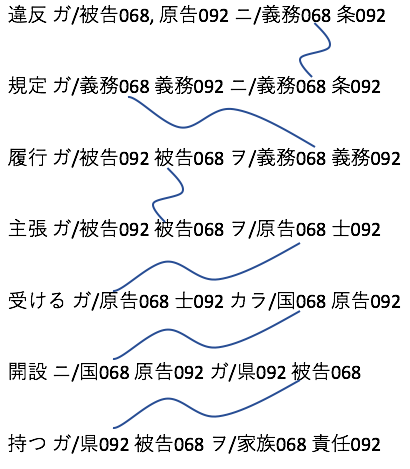
\includegraphics[width=250pt]{./pictures/0403-3.png}
\caption{Part of Descriptive patterns between similar documents}
\end{figure}

\newpage
\section{Conclusion}
In Experiment 1, we verify the feasibility of KeyGraph, only with high KeyScore nouns, the connection between events won't be broken. Applying KeyGraph Algorithm can improve the efficiency and it is safe to use the result and disregard low KeyScore nouns.\\
In Experiment 2, we found that MFC by CLIQUE will work very slow if the input data become very large, as we know maximal clique problem is an NP complete problem. To be honest, CLIQUE may be the fastest way to find maximal cliques, and in the situation of document number less than 50, the runtime of algorithm is acceptable.\\
In Experiment 3, we apply our algorithm to 2 short Japanese stories. Although there are only four closures, we can still find the similarity classes between them. That means our algorithm can deal with very short documents.\\
In Experiment 4, we have done 3 different things. According to the whole result of these experiments, we can say, it is possible for our algorithm to find similar documents among multiple documents. And we can build the descriptive patterns using the result of our experiment. To build descriptive patterns, we can use the proposed method we have mentioned in the section of beam search. It may be a convenient algorithm to try in the future.
\chapter{Summary and Future Work}
\section{Ssummary}
In this research, we use KNP tool to obtain event data as a list of verb-noun pairs:$v(c_1:n_1,n_2:n_2,...)$. we also use the output of KNP and KeyGraph to extract keywords. We have done an experiment to verify the feasibility of KeyGraph. After all the pre-work, we obtain maximal closures which can be used to build descriptive patterns by CLIQUE algorithm. We manual pick some candidates of descriptive patterns, that means maximal closure can be a possible way to extract all descriptive patterns. Limited by time and ability we didn't get the exactly descriptive pattern, but we have proposed a possible way of beam search to extract some descriptive patterns. It becomes a future work in my future research.
\section{Future Work}
In our research, we proposed a possible method to obtain possible descriptive patterns from maximal closures but limited by time and ability we didn't get all the exactly descriptive pattern. In the future research, we can continue the topic and find some feasible and efficient method to re-construct descriptive patterns. \\
As a fact, we can define each maximal closure a degree by the importance of nouns, and use a top-n clique algorithm to extract ranked maximal closures. This method may improve the effciency of the algorithm, and it is very helpful for our research.\\
In our research, we use 10 main cases from KNP tool, actually, there are over 20 kinds of cases that can be extracted. If we can extend the cases set, using some deep cases like location, agent, and others can also a powerful method to improve our research.\\
We have done some passive voice processing in the experiment, such as changing the case, the passive voice into an active voice. But there is another case that we did not consider like borrowing. In this case, the subject and goal of the action are exactly the opposite. If we forget to deal with this particular situation, we may completely wrong the nouns of these verbs, leading to further mistakes. Find out the grant relationship also can improve the result of our research.
\newpage
\section*{Acknowledgement}
I would like to express my gratitude to all those who helped me during the writing of this thesis. My deepest gratitude goes first and foremost to Professor Haraguchi, my supervisor, for his constant encouragement and guidance. He has walked me through all the stages of the writing of this thesis. Without his consistent and illuminating instruction, this thesis could not have reached its present form as a foreign student.\\
In addition, I also want to extend my gratitude to Professor Yoshioka and Dr. Okubo, who is always kind to me since I joined our laboratory. They alway give me sincere advice.\\
Finally, I would like to thank all the people who supported me in my university life so far.
\renewcommand\bibname{References}
\begin{thebibliography}{9}

%\bibitem{}
%
%
%
\bibitem{}\begin{CJK}{UTF8}{ipxm}王叡鵬,原口誠: 構造類似性の列挙問題\end{CJK}, FIT 2017, Tokyo, Sep 2017

\bibitem{}\begin{CJK}{UTF8}{ipxm}全新受事件の最近5年間の推移『全裁判所』\end{CJK}, Courts in Japan, http://www.courts.go.jp/

\bibitem{}\begin{CJK}{UTF8}{ipxm}判例データーベース第一法規株式会社『D1-law.com』\end{CJK}, http://www.d1-low.com/.

\bibitem{}\begin{CJK}{UTF8}{ipxm}構文解析システム\end{CJK}KNP, http://nlp.ist.i.kyoto-u.ac.jp/index.php?KNP 


\bibitem{}Yukio Ohsawa,Nels E. Benson and Masahiko Yachida, KeyGraph: Automatic Indexing by Co-occurrence Graph based on Building Construction Metaphor,  pp.391-400, 1999.

\bibitem{}Etsuji Tomita, Akira Tanaka and Haruhisa Takahashi, The worst-case time complexity for generating all maximal cliques and computational experiments, Elsevier B.V., 2006.

\bibitem{}Takashi Nakagawa and Etsuji Tomita, An algorithm for generating all Maximal Bipartite Cliques Based on CLIQUES that Generates All Maximal Cliques, IPSJ SIG Technical Report, 2006.

\bibitem{}C. Bron, J. Kerbosch, Algorithm 457, finding all cliques of an undirected graph, Comm. ACM 16 (1973) 575–577.

\bibitem{}Swaminathan,K., Tau: A domain-independent approach to information extraction from natural language documents. DARPA workshop on document management, Palo Alto, 1993.

\bibitem{}Ryohei Sasano and Sadao Kurohashi.
A Discriminative Approach to Japanese Zero Anaphora Resolution with Large-scale Lexicalized Case Frames, In Proceedings of the 5th International Joint Conference on Natural Language Processing (IJCNLP2011), pp.758-766, 2011.
\bibitem{}G.D.Plotkin A Note on Inductive Generalization, Machin Intelligence Vol.5, 153--163, 1970
\bibitem{}\begin{CJK}{UTF8}{ipxm}喜多陵\end{CJK}, \begin{CJK}{UTF8}{ipxm}記述の構造類似性に基づく法的観点と判例のマッチング\end{CJK}, 修士論文, Hokkaido University, Graduate School of Information Science and Technology, 2014.

\bibitem{}Xiaolong Zhang, Towards a Detection of Descriptive Similarities among Multiple Precedents Based on Formal Concept Analysis, Master Thesis, Hokkaido University, Graduate School of Information Science and Technology, 2016.


\end{thebibliography}

\end{document}
